\chapter[HASIL DAN PEMBAHASAN]{\\HASIL DAN PEMBAHASAN}

\section{Perancangan Front End}
Pada tahap perancangan Frontend, penulis menggunakan HTML, CSS, dan Javascript yang diimplementasikan pada framework Laravel. Dari rancangan desain yang telah dibuat, terdapat dua halaman utama dan beberapa function yang mengeksekusi program, seperti fetch API, menampilkan dropdown yang berisi parameter dari API yang di-generate, membuat visualisasi dengan library, dan lainnya. 

\subsection{Halaman Utama}
Pada halaman ini, terdapat beberapa fitur dan fungsi Javascript untuk menjalankan fungsionalitas website. Potongan kode berikut berfungsi untuk men-generate keys yang ada di dalam API yang diinputHakan dari tampilan yang dibuat menggunakan HTML. 
	\begin{figure}[H]
	\centering
	\includegraphics[width=0.8\linewidth]{gambar/Pembahasan/generate API.png}
	\caption{Generate API}
	\label{Generate API}
\end{figure}

Fungsi yang ada pada potongan kode diatas adalah fungsi generateAPI(). Script Javascript yang disusun untuk fungsi tersebut adalah seperti berikut :
	\begin{figure}[H]
	\centering
	\includegraphics[width=0.8\linewidth]{gambar/Pembahasan/fungsi Generate.png}
	\caption{Fungsi Generate API}
	\label{Fungsi Generate API}
\end{figure} 

Kode JavaScript di atas dibuat untuk mengambil data dari API yang dimasukkan oleh pengguna melalui kolom input, lalu menampilkan daftar checkbox berdasarkan kunci-kunci (keys) dari data yang diperoleh. Jika tidak ada input API pada kolom dengan id = “api-input”, sistem akan menampilkan peringatan agar pengguna memasukkan URL yang valid.\\
 
Berikutnya, API akan diambil dengan menggunakan fungsi fetch(). Fetch sendiri merupakan sebuah fungsi bawaan Javascript yang digunakan mengambil data dari sumber eksternal, seperti API, file JSON, atau file lain yang tersedia di server.  Jika respons API gagal, maka sistem akan menampilkan error dan menghentikan proses lebih lanjut. Namun, jika data berhasil diperoleh, sistem akan mengolahnya untuk mendapatkan daftar keys. Setelah daftar keys diperoleh, untuk setiap key, sistem akan menambahkan elemen input bertipe checkbox kemudian tiap checkbox diberi atribut id dan value sesuai dengan key yang bersangkutan sehingga data tersimpan sebagai pasangan key-value. Setelah itu, elemen-elemen ini akan ditempatkan dalam div utama yang memiliki id="api-keys", sehingga checkbox dapat ditampilkan di halaman main page. 
Jika terdapat kesalahan saat mengambil data dari API, error akan dicatat dan ditampilkan di console, dan sistem akan menampilkan peringatan bahwa pengambilan data gagal melalui alert. Dengan fitur ini, pengguna dapat melihat keys pada API secara langsung dan dapat memilih key yang dibutuhkan melalui checkbox yang disediakan. 
	\begin{figure}[H]
	\centering
	\includegraphics[width=0.8\linewidth]{gambar/Pembahasan/use Feature.png}
	\caption{Generate API}
	\label{Fungsi Use Feature}
\end{figure}
Setelah pengguna memilih keys dari checkbox dan menekan tombol “use features” dengan id=“addfeatures”, data akan disimpan di localStorage untuk ditampilkan pada halaman visualisasi. 


\subsection{Halaman Visualisasi}
Pada halaman visualisasi, kode dari fitur dan fungsi digunakan untuk menampilkan dan menambahkan visualisasi secara dinamis dalam sebuah container. 
\begin{enumerate}[label={\alph*.}]
	\item Fungsi Log Render \\
Kode berikut merupakan fungsi untuk mencatat dan menyimpan log waktu rendering setiap grafik yang dihasilkan oleh library visualisasi data. Fungsi ini memastikan bahwa setiap proses pembuatan dan pembaruan grafik terdokumentasi dengan baik, sehingga dapat digunakan untuk analisis performa dan evaluasi efisiensi rendering secara berkala.
		\begin{figure}[H]
	\centering
	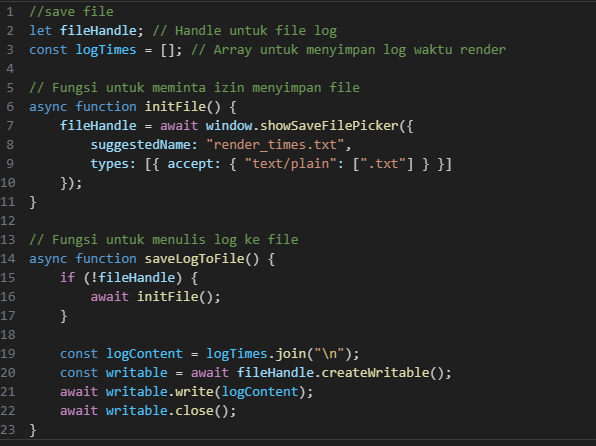
\includegraphics[width=0.8\linewidth]{gambar/Pembahasan/menyimpan log.png}
	\caption{Fungsi Menyimpan Log Render}
	\label{Fungsi Menyimpan Log Render}
	\end{figure} 
	\item Fungsi Fetch Data\\
	Kode JavaScript pada gambar berikut berfungsi untuk mengambil data sensor dari API yang disimpan secara lokal secara berkala dan memperbarui tampilan grafik dengan data terbaru. 
		\begin{figure}[H]
		\centering
		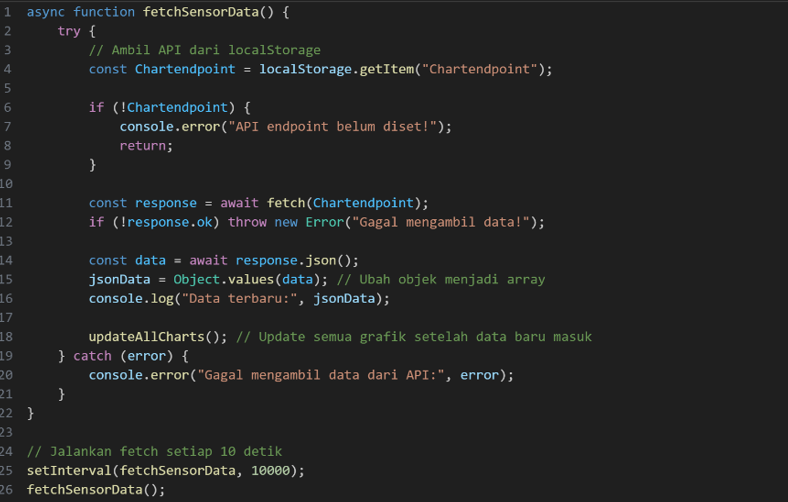
\includegraphics[width=0.8\linewidth]{gambar/Pembahasan/Fungsi Fetch Data.png}
		\caption{Fungsi Fetch Data}
		\label{Fungsi Fetch Data}
	\end{figure} 
	
	Data akan diperbarui dengan menggunakan fungsi bawaan setInterval(fetchSensorData, 10000) yang akan memanggil fetchSensorData() setiap 10 detik. Pada konteks ini, fetchSensorData() bersifat asinkron untuk memastikan proses pengambilan data tidak menghambat eksekusi kode lainnya. Jika respons dari API tidak berhasil, fungsi akan menampilkan eror. 
	Jika data berhasil diambil, tampilan grafik akan diperbarui dengan pemanggilan fungsi updateAllCharts(). Fungsi ini akan memanggil fungsi UpdateChart untuk memperbarui visualisasi pada id chart tertentu.
		\begin{figure}[H]
		\centering
		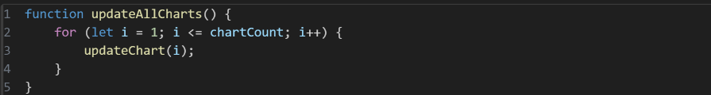
\includegraphics[width=0.8\linewidth]{gambar/Pembahasan/update all data.png}
		\caption{Memperbarui Data pada Chart}
		\label{Memperbarui Data pada Chart}
	\end{figure} 

	
	\item fungsi AddNewVisualization()\\
	Ketika tombol “add new visualization” pada halaman ditekan, fungsi addNewVisualization() akan menambahkan elemen baru ke dalam div dengan id='visualizations' berupa template chart.
		\begin{figure}[H]
		\centering
		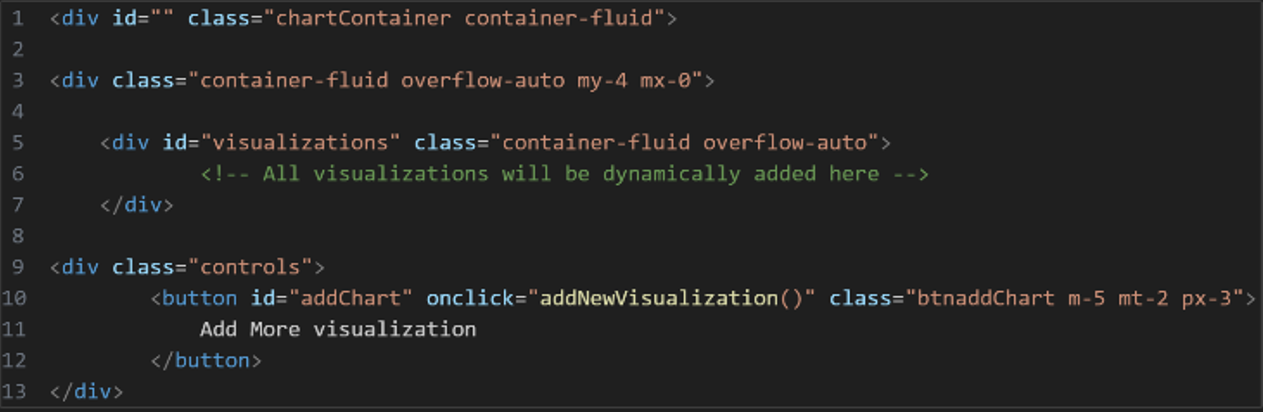
\includegraphics[width=0.8\linewidth]{gambar/Pembahasan/button new visualization.png}
		\caption{Potongan Kode Pada Button New Visualization}
		\label{Potongan Kode Pada Button New Visualization}
	\end{figure}
	
	Tombol dengan id addChart pada event onclick diatas, akan mengeksekusi fungsi addNewVisualization() berikut :
	
	\begin{figure}[H]
		\centering
		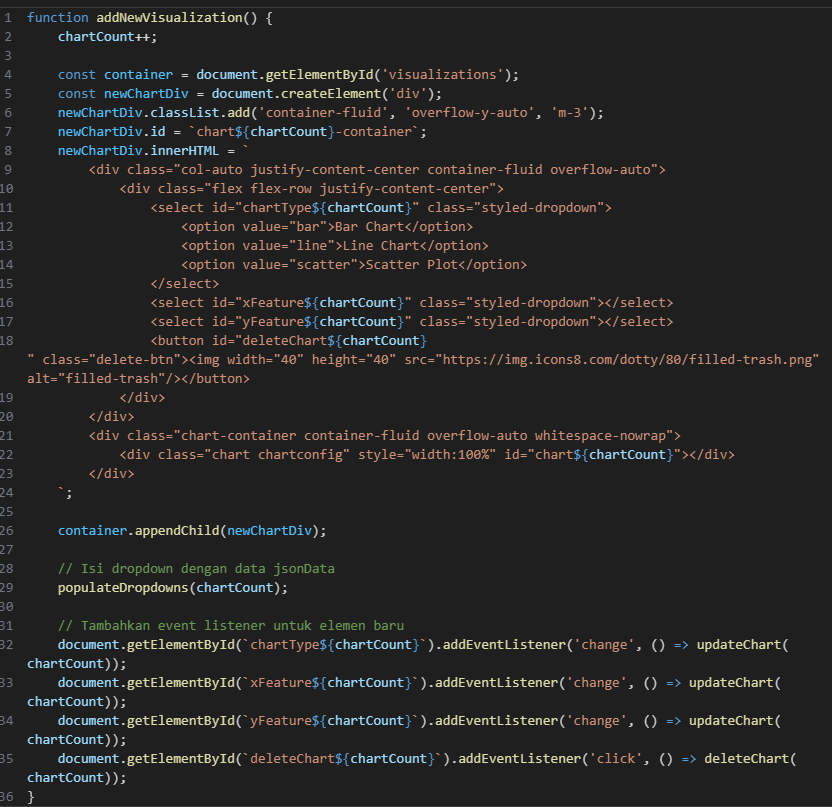
\includegraphics[width=0.8\linewidth]{gambar/Pembahasan/Fungsi new visualization.png}
		\caption{Fungsi untuk Membuat Visualisasi Baru}
		\label{Fungsi untuk Membuat Visualisasi Baru}
	\end{figure}
	Setiap kali fungsi addNewVisualization() dipanggil, variabel chartCount akan menambahkan elemen baru pada wadah div dengan id= “visualizations”. Di dalam elemen <div> yang baru dibuat terdapat dua dropdown yang memungkinkan pengguna memilih tipe grafik (bar, line, atau scatter plot) dan fitur yang akan divisualisasikan. Setiap dropdown memiliki id yang mengandung nilai chartCount agar tidak mengubah visualisasi yang lain ketika terdapat perubahan. Selain itu, terdapat tombol delete yang memungkinkan pengguna menghapus visualisasi tertentu dengan mengklik ikon “trash”.\\
	Setelah struktur HTML untuk visualisasi baru selesai dibuat, elemen tersebut dimasukkan ke dalam container utama menggunakan appendChild(). Fungsi populateDropdowns(chartCount) kemudian dipanggil untuk mengisi dropdown dengan data yang sesuai. 
	
	\item Fungsi PopulateDropdown()\\
	Untuk menampilkan dropdown yang datanya diambil dari data-data API, diperlukan fungsi populateDropdowns(chartCount) seperti pada gambar berikut : 
		\begin{figure}[H]
		\centering
		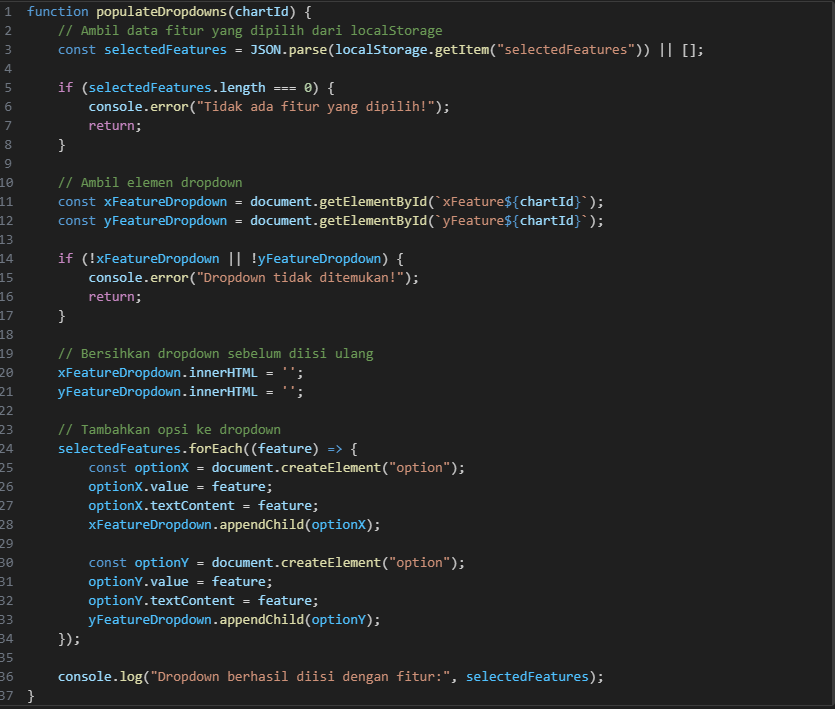
\includegraphics[width=0.8\linewidth]{gambar/Pembahasan/fungsi_populate_dropdown.png}
		\caption{Fungsi untuk Populate Dropdown}
		\label{Fungsi untuk Populate Dropdown}
	\end{figure}
	fungsi ini mengambil data fitur yang telah dipilih sebelumnya dari localStorage.getItem("selectedFeatures"). Jika tidak ada data yang tersimpan, maka variabel selectedFeatures akan berisi array kosong dan sistem akan menunjukkan eror pada console. Kemudian, fungsi ini akan mencocokkan elemen dropdown dengan chartid. Jika salah satu elemen tidak ditemukan, akan muncul pesan eror di console, dan fungsi akan berhenti. Jika elemen dropdown sesuai dengan chartid dan selectedFeatures tidak kosong, selanjutnya fungsi akan menambahkan keys ke dalam dropdown berdasarkan daftar selectedFeatures.
	\item Fungsi CreateChart()\\
	Fungsi createChart() merupakan fungsi yang digunakan untuk menambahkan kode visualisasi sesuai dengan library yang akan diujicobakan.
	\item fungsi UpdateChart()
	 Merupakan fungsi yang digunakan untuk memperbarui grafik secara dinamis berdasarkan data JSON yang ada atau saat fitur pada dropdown diubah. Fungsi ini juga disesuaikan dengan library yang diuji cobakan. 
	fungsi ini mengambil input dari elemen HTML untuk menentukan jenis grafik (chartType), fitur yang akan digunakan sebagai sumbu x (xFeature), dan fitur untuk sumbu y (yFeature) dari array JSON. Data untuk sumbu x disimpan dalam variabel labels, sedangkan data untuk sumbu y disimpan dalam chartData. Keduanya diperoleh menggunakan map(), yang mengambil nilai dari properti yang sesuai dalam objek JSON berdasarkan fitur yang dipilih. Setelah data diperoleh, fungsi createChart(chartId, chartType, labels, chartData) akan dipanggil untuk membuat atau memperbarui grafik dengan data terbaru. 
	\item Fungsi DeleteChart()\\
	Fungsi ini akan memeriksa grafik yang akan dihapus berdasarkan id-nya. Kemudian, grafik akan dihapus dengan fungsi destroy(). Referensi terhadap grafik tersebut juga akan dihapus dari objek chartInstances menggunakan delete chartInstances[chartId]. 
		 \begin{figure}[H]
		\centering
		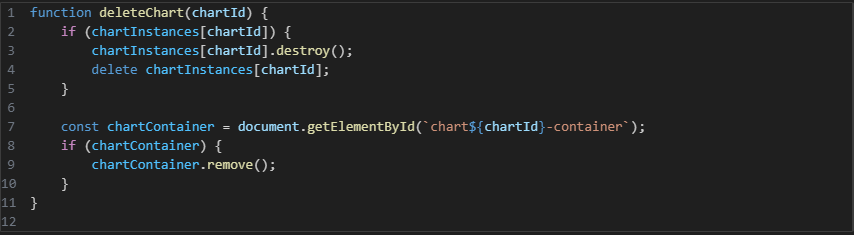
\includegraphics[width=0.8\linewidth]{gambar/Pembahasan/delete-chart.png}
		\caption{Fungsi Delete Chart}
		\label{Fungsi Delete Chart}
		\end{figure}
	\end{enumerate}
	
\section{Implementasi Library}
\subsection{Implementasi Pada Chart.js}
Tahap awal implementasi pada Chart.js dilakukan dengan pembuatan struktur Chart.js pada fungsi createChart(). Fungsi utama dalam kode ini adalah createChart(chartId, chartType, labels, data), yang menerima empat parameter, yaitu chartId untuk memberi id grafik yang akan dibuat, chartType untuk mendefinisikan jenis chart yang akan dibuat, labels untuk menandakan sumbu x, dan variabel data yang akan ditampilkan di dalam grafik sumbu y,  Konfigurasi grafik mencakup tampilan responsif (responsive: true) agar grafik dapat menyesuaikan ukuran layar, skala sumbu x dan y (scales) yang mengatur tampilan label, rotasi teks, serta padding, layout (layout) untuk mengatur jarak padding grafik terhadap batas kanvas, dan Fitur tooltip untuk menampilkan informasi saat pengguna mengarahkan kursor ke grafik.
\begin{enumerate}
	\item Inisialisasi Variabel
	\begin{figure}[H]
		\centering
		\includegraphics[width=0.8\linewidth]{gambar/Pembahasan/Init variabel cjss.png}
		\caption{Inisialisasi Variabel dan Pengukuran Performa}
		\label{Inisialisasi Variabel dan Pengukuran Performa}
	\end{figure}
	
	\item Menentukan Tipe Chart
	\begin{figure}[H]
		\centering
		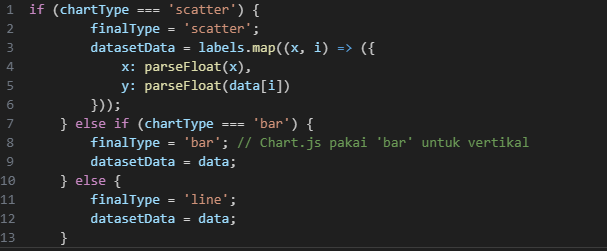
\includegraphics[width=0.8\linewidth]{gambar/Pembahasan/type visual.png}
		\caption{Potongan Kode untuk Menentukan Jenis Visualisasi}
		\label{Potongan Kode untuk Menentukan Jenis Visualisasi}
	\end{figure}
	Potongan kode diatas berfungsi untuk menyesuaikan jenis grafik dan format data yang akan ditampilkan menggunakan Chart.js. Jenis grafik yang akan ditampilkan disesuaikan dengan tipe visualisasi yang dipilih. Pada kondisi ini, data tetap digunakan dalam bentuk array numerik tanpa perlu mengubah strukturnya. Apabila jenis grafik yang dipilih bukan scatter maupun bar, maka secara bawaan tipe grafik diatur menjadi 'line' dengan data yang juga tetap berupa array numerik. 
	
	\item Pembuatan Chart
		\begin{figure}[H]
		\centering
		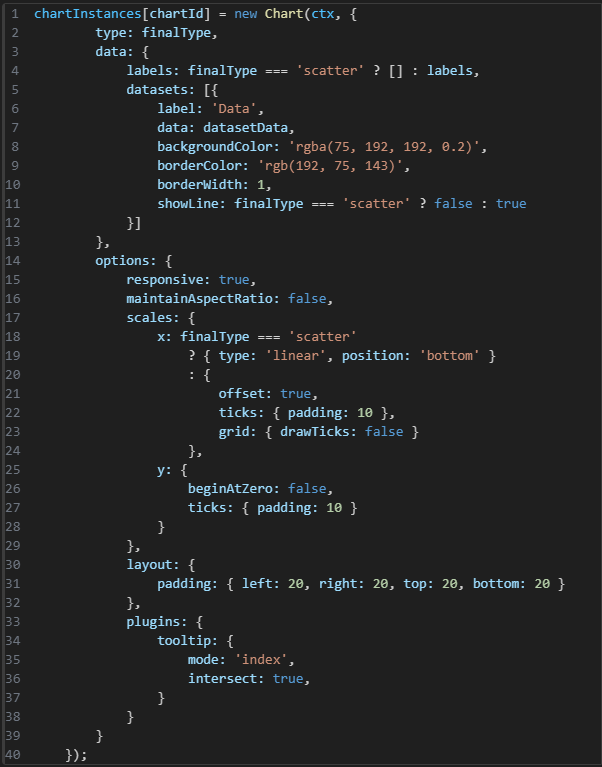
\includegraphics[width=0.8\linewidth]{gambar/Pembahasan/Chartinstance cjs.png}
		\caption{Potongan Kode untuk Pembuatan Chart}
		\label{Potongan Kode untuk Pembuatan Chart}
	\end{figure}
	Potongan kode di atas merupakan bagian dari pembuatan objek grafik baru dengan Chart.js, yang disimpan di dalam `chartInstances` menggunakan `chartId` sebagai \textit{identifier}. Pada bagian `type`, nilai `finalType` digunakan untuk menentukan jenis grafik sesuai hasil logika sebelumnya. Struktur data grafik juga menyesuaikan: jika tipe grafik scatter, maka `labels` dibiarkan kosong karena Chart.js tidak memerlukan sumbu kategori untuk scatter plot, sedangkan pada tipe lain seperti bar dan line, `labels` diisi dengan data kategori sumbu X. Selain itu, pengaturan dataset disesuaikan melalui properti `showLine`, yang akan bernilai `false` khusus untuk scatter agar titik data tidak dihubungkan oleh garis, dan `true` untuk jenis grafik lainnya. Pada bagian `options`, properti `responsive` dan `maintainAspectRatio` memastikan grafik tetap menyesuaikan ukuran layar dengan proporsi yang diatur. Bagian `scales` juga dibuat fleksibel: jika tipe scatter, maka sumbu X diatur sebagai sumbu linear pada posisi bawah. Sedangkan pada tipe lainnya, sumbu X diformat sebagai sumbu kategori dengan pengaturan tampilan tambahan seperti jarak dan grid. Bagian `layout` digunakan untuk memberikan jarak tepi di sekitar area grafik, sedangkan `plugins.tooltip` mengatur perilaku penampilan tooltip agar lebih informatif saat pengguna berinteraksi dengan grafik. Dengan rangkaian pengaturan ini, grafik yang ditampilkan akan memiliki format visual yang benar sesuai tipe data dan kebutuhan pengguna, serta tetap responsif terhadap perubahan tampilan layar.
	
	\item Fungsi Update Chart\\
		\begin{figure}[H]
		\centering
		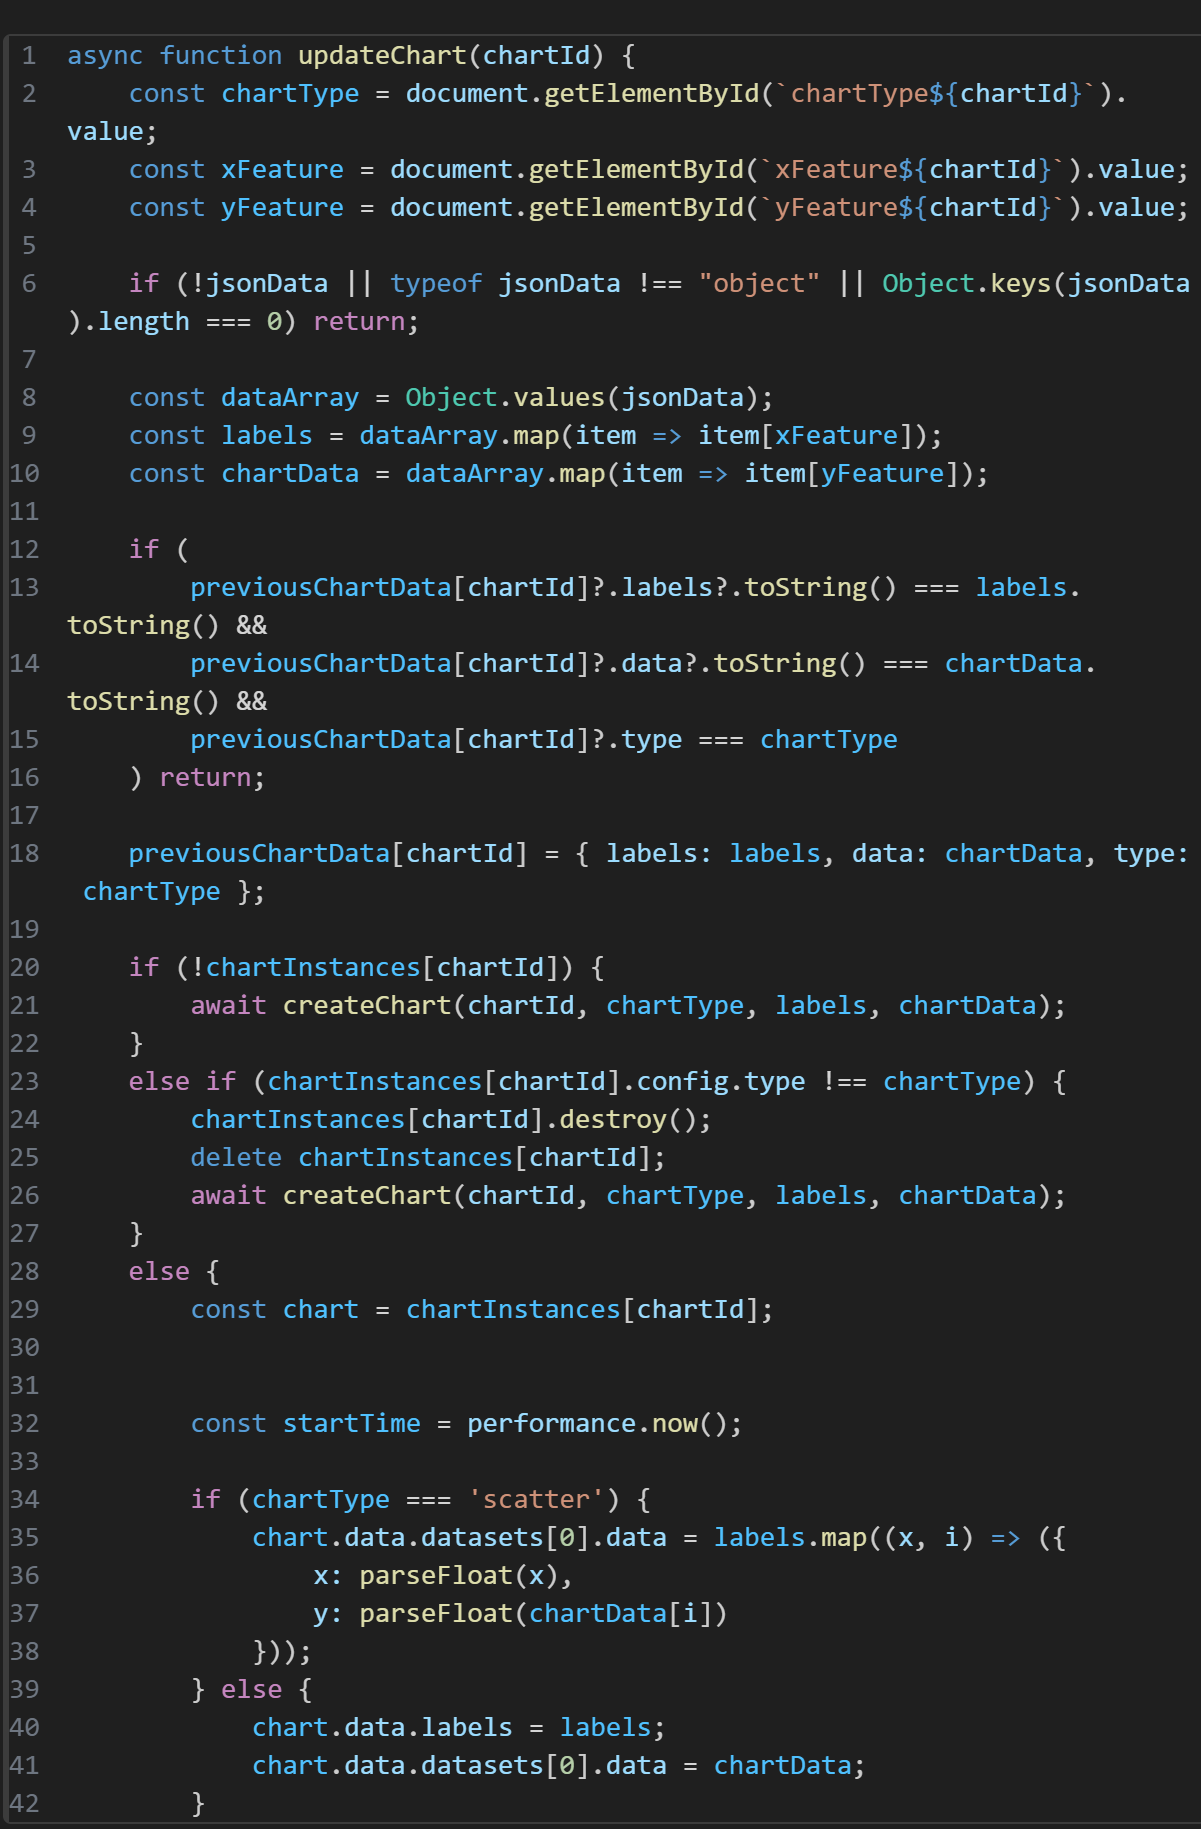
\includegraphics[width=0.8\linewidth]{gambar/Pembahasan/update data cjs.png}
		\caption{Potongan Kode untuk Pembuatan Chart}
		\label{Potongan Kode untuk Pembuatan Chart}
	\end{figure}
	
	Fungsi `updateChart` ini pada dasarnya bertugas memastikan setiap grafik yang tampil selalu mengikuti data sensor terbaru dan pengaturan yang dipilih pengguna. Fungsi akan mengidentifikasi tipe grafik,fitur pada sumbu x, dan fitur pada sumbu y dari dropdown yang berkaitan dengan ID grafik tertentu.\\
	Jika grafik belum ada sama sekali, grafik baru dibuat. Jika tipe grafik diubah, grafik lama dihapus dan diganti dengan grafik baru agar sesuai tipe, dan jika hanya datanya yang berubah, label dan isi datanya diperbarui tanpa perlu membongkar grafik dari awal. 
\end{enumerate}

\subsection{Implementasi Pada D3}
Implementasi pada D3.js dilakukan dengan mengubah fungsi CreateChart() pada kode yang telah dibuat sebelumnya. Penjelasan kode yang diubah adalah sebagai berikut : \\
\begin{enumerate}
	\item Melakukan inisialisasi dan mengatur ukuran chart. Kemudian mengubah sumbu x menjadi scale band yang dapat menerima data kategorikal dan sumbu y menjadi linear agar dapat menampilkan data numerik kontinyu. Kemudian membuat sumbu x dan sumbu y dengan menerapkan beberapa atribut. Seperti pada sumbu x, atribut yang diterapkan adalah translate untuk memindahkan sumbu menjadi dibaagian bawah, memutar teks pada sumbu x dan mengatur font, serta memberikan filter untuk menampilkan keterangan di sumbu x. Adapun atribut yang diterapkan di sumbu y adalah d3.axisLeft tickValues(uniqueYValues) membatasi label sumbu y hanya pada nilai-nilai tertentu.
	\begin{figure}[H]
		\centering
		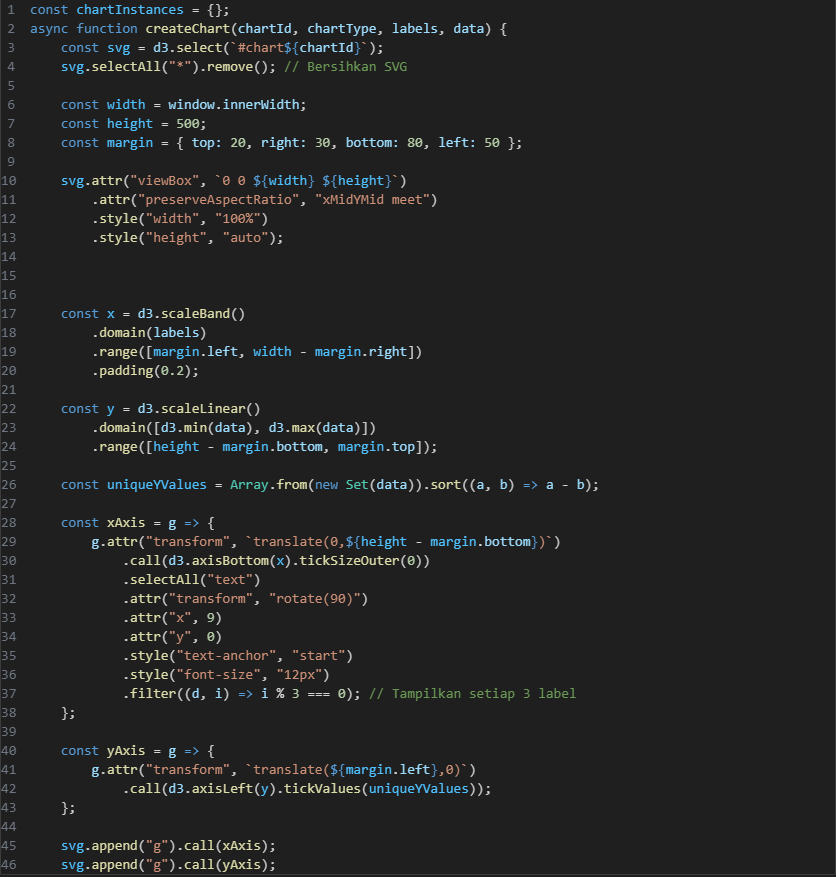
\includegraphics[width=0.8\linewidth]{gambar/Pembahasan/create axis d3.png}
		\caption{Membuat Sumbu Pada D3}
		\label{Membuat Sumbu Pada D3}
	\end{figure}
	\item Menyediakan tooltip yang akan ditampilkan saat kursor di hover ke titik data pada chart.
	\begin{figure}[H]
		\centering
		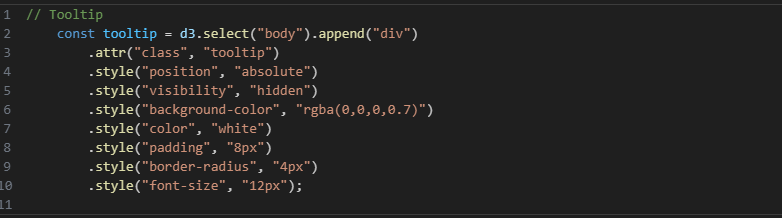
\includegraphics[width=0.8\linewidth]{gambar/Pembahasan/Create Tooltip.png}
		\caption{Potongan Kode untuk Membuat Tooltip }
		\label{Potongan Kode untuk Membuat Tooltip }
	\end{figure} 
	\item Menambahkan visualisasi berdasarkan jenis grafik yang akan dipilih (line chart, bar chart, atau scatter plot). Kode berikut membuat grafik garis (line chart). Pertama, dibuat jalur garis menggunakan d3.line() berdasarkan data dan label yang dipetakan ke sumbu x dan y. Kemudian, titik-titik data ditampilkan sebagai titik merah. Setiap titik memiliki interaksi tooltip yang muncul saat pointer diarahkan ke titik dan akan menampilkan informasi sumbu x dan sumbu y.
	\begin{figure}[H]
		\centering
		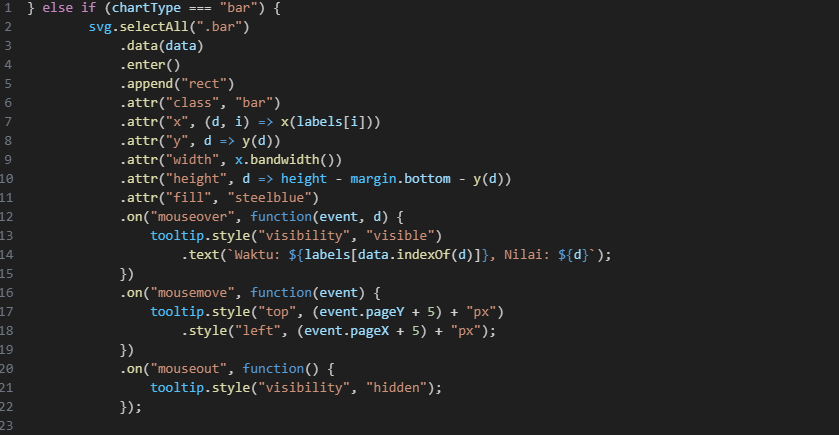
\includegraphics[width=0.8\linewidth]{gambar/Pembahasan/implementasi bar chart.png}
		\caption{Potongan Kode untuk Mengimplementasikan Line Chart}
		\label{Potongan Kode untuk Mengimplementasikan Line Chart}
	\end{figure}
	\item Membuat grafik diagram batang dengan elemen rect. Pada kode berikut posisi batang diatur dengan .attr("x", ...) berdasarkan label dan skala data x. Tinggi batang dihitung dari selisih tinggi SVG dan posisi data pada sumbu y, sementara lebar batang diambil dari x.bandwidth(). 
	\begin{figure}[H]
		\centering
		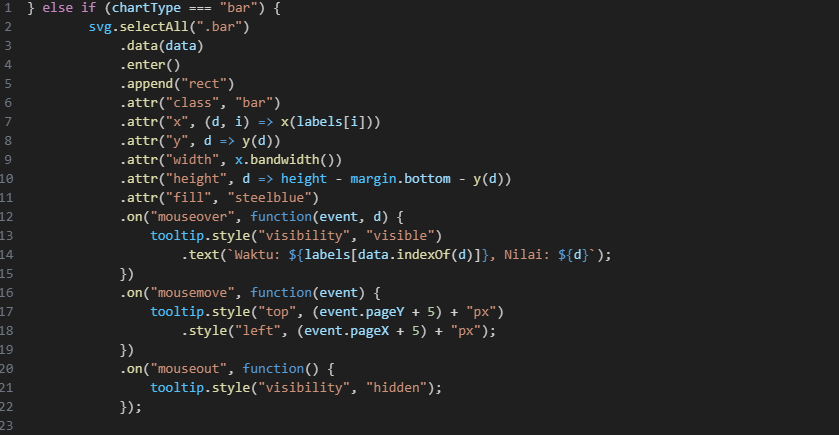
\includegraphics[width=0.8\linewidth]{gambar/Pembahasan/implementasi bar chart.png}
		\caption{Potongan Kode untuk Mengimplementasikan Bar Chart}
		\label{Potongan Kode untuk Mengimplementasikan Bar Chart}
	\end{figure}
	\item Membuat grafik scatter plot, dengan menentukan posisi x dan y. Masing-masing titik digambar sebagai lingkaran berwarna kuning dengan garis tepi hitam. Tooltip interaktif juga digunakan, sama seperti pada grafik batang, untuk menunjukkan informasi detail saat pointer diarahkan ke titik.
	\begin{figure}[H]
		\centering
		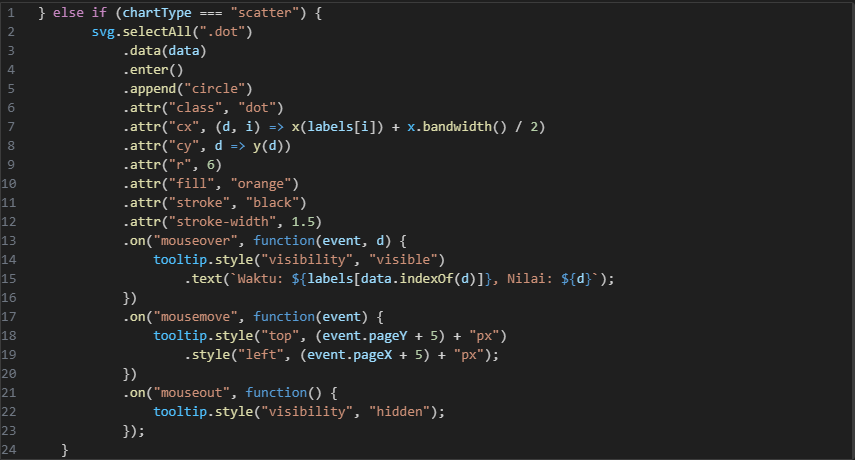
\includegraphics[width=0.8\linewidth]{gambar/Pembahasan/implementasi scatter plot.png}
		\caption{Potongan Kode untuk Mengimplementasikan Scatter Plot}
		\label{Potongan Kode untuk Mengimplementasikan Scatter Plot}
	\end{figure}
	
	\item Fungsi Update Pada D3
		\begin{figure}[H]
		\centering
		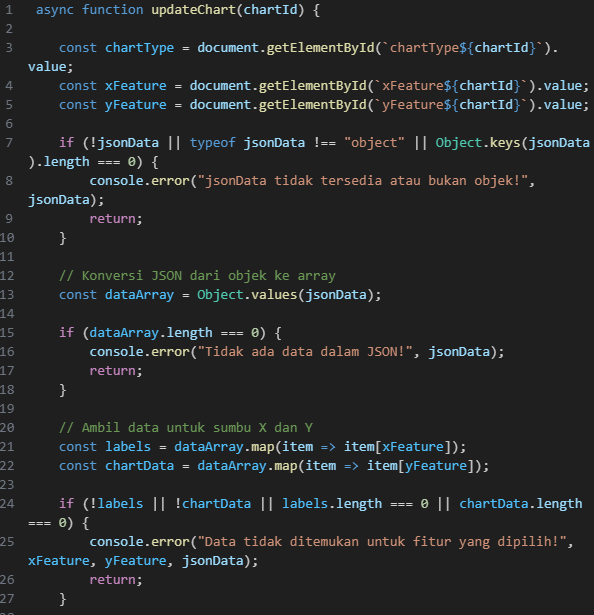
\includegraphics[width=0.8\linewidth]{gambar/Pembahasan/Fungsi Update D3.png}
		\caption{Fungsi untuk Memperbarui Chart D3}
		\label{Fungsi untuk Memperbarui Chart D3}
	\end{figure}
	Fungsi diatas akan mengambil informasi dari elemen HTML berupa tipe grafik, nama fitur untuk sumbu X, dan fitur untuk sumbu Y berdasarkan ID grafik yang sedang diproses. Setelah itu, fungsi memeriksa apakah jsonData yang berisi data sensor sudah valid, berupa objek, dan memiliki isi. Jika data tidak ada atau tidak sesuai format, fungsi akan menghentikan proses dan mencatat pesan kesalahan ke konsol untuk memudahkan pengecekan. Kemudian objek JSON diubah menjadi array agar lebih mudah diolah. Jika array ini kosong, berarti tidak ada data valid yang dapat divisualisasikan, sehingga fungsi kembali membatalkan proses dan menampilkan error. Kemudian, data untuk sumbu X dan Y diambil masing-masing dengan melakukan mapping ke array fitur X menjadi label, dan fitur Y menjadi data nilai.	
\end{enumerate}



\subsection{Implementasi Pada Highcharts}
Implementasi Highcharts dilakukan pada fungsi CreateChart() dengan menambahkan kode berikut.\\
\begin{enumerate}
\item Implementasi Kontainer Grafik\\
 Pertama, kode membuat id kontainer grafik. Jika grafik dengan chartId yang sama sudah pernah dibuat sebelumnya, maka grafik lama akan dihapus menggunakan fungsi destroy() untuk mencegah duplikasi. 
		\begin{figure}[H]
	\centering
	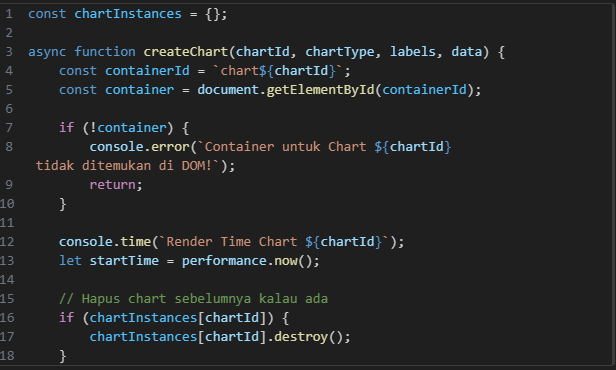
\includegraphics[width=0.8\linewidth]{gambar/Pembahasan/Init Highcharts.png}
	\caption{Potongan Kode untuk Kontainer Grafik}
	\label{Potongan Kode untuk Kontainer Grafik}
\end{figure}
\item Implementasi ChartOptions\\
Selanjutnya, objek chartOptions disusun sebagai konfigurasi grafik. Pada bagian chart, properti renderTo menunjukkan elemen HTML yang menjadi wadah grafik, sementara type diisi dengan tipe grafik dari variabel highchartsType yang sudah ditetapkan. 
		\begin{figure}[H]
	\centering
	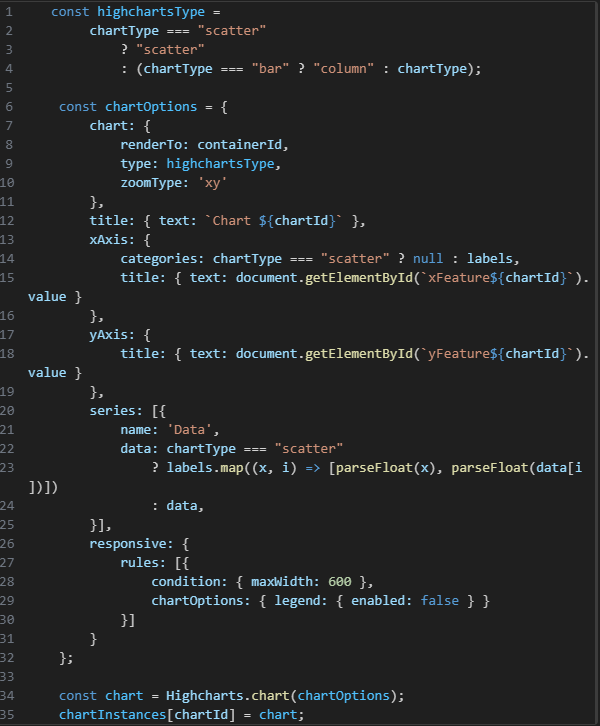
\includegraphics[width=0.8\linewidth]{gambar/Pembahasan/Membuat chart highcharts.png}
	\caption{Potongan Kode untuk Membuat Grafik Highcharts}
	\label{Potongan Kode untuk Membuat Grafik Highcharts}
\end{figure}

Properti zoomType diaktifkan agar pengguna dapat melakukan pembesaran tampilan grafik pada sumbu horizontal dan vertikal. Untuk sumbu X (xAxis), apabila grafik berjenis scatter, properti categories diatur null karena scatter plot memanfaatkan nilai numerik langsung, bukan kategori. Sebaliknya, untuk jenis grafik lain, labels digunakan sebagai penanda kategori. Judul pada sumbu X dan Y diatur berdasarkan input fitur X dan Y yang dipilih pengguna melalui elemen HTML.

Bagian series berfungsi menentukan data yang akan divisualisasikan. Jika grafik bertipe scatter, data diolah menjadi pasangan nilai [x, y] dengan format numerik melalui parseFloat. Untuk tipe grafik lain, data digunakan sebagaimana adanya. Di bagian responsive, terdapat aturan tambahan yang akan menyembunyikan legenda grafik secara otomatis jika lebar layar di bawah 600 piksel, sehingga tampilan tetap rapi pada perangkat berlayar kecil. Kemudian, perintah Highcharts.chart(chartOptions) akan merender grafik sesuai pengaturan tersebut ke dalam halaman. Hasil grafik ini kemudian disimpan ke dalam chartInstances[chartId] agar dapat diakses dan diperbarui. 

\item Update Highcharts\\
 Fungsi updateChart yang berfungsi untuk memperbarui data grafik berdasarkan fitur yang dipilih. Langkah kerjanya dimulai dengan mengambil jenis grafik serta nama fitur untuk sumbu X dan Y dari elemen HTML. Kemudian, fungsi akan memvalidasi jsonData. Selanjutnya, data JSON dikonversi menjadi array, lalu dipecah menjadi data sumbu X (labels) dan data sumbu Y (chartData). Jika hasil ekstraksi data kosong atau gagal, fungsi juga akan berhenti sambil menampilkan pesan error. Terakhir, jika semua valid, data tersebut akan dipakai untuk membuat atau memperbarui grafik.
 		\begin{figure}[H]
 	\centering
 	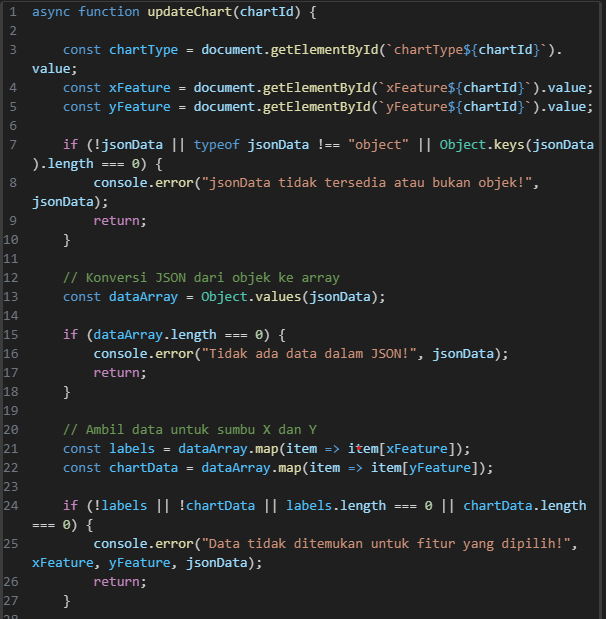
\includegraphics[width=0.8\linewidth]{gambar/Pembahasan/Update Highcharts.png}
 	\caption{Potongan Kode untuk Memperbarui Grafik Highcharts}
 	\label{Potongan Kode untuk Memperbarui Grafik Highcharts}
 \end{figure}
\end{enumerate}


\section{Pengukuran Performa Rendering}
Pada bagian ini, dilakukan pengukuran performa rendering untuk menilai seberapa efisien dan responsif library dalam menampilkan data visualisasi. Pengujian dilakukan dengan menggunakan beberapa skenario jumlah data yang ditampilkan melalui line chart untuk mengamati waktu yang dibutuhkan dalam merender grafik ke layar. Proses pengukuran dilakukan dengan mencatat waktu rendering sejak inisialisasi data hingga grafik ditampilkan secara penuh di DOM. Analisis ini bertujuan untuk memberikan gambaran kuantitatif mengenai kemampuan library dalam menangani berbagai skenario penggunaan, serta menjadi dasar perbandingan dengan library visualisasi data lainnya. Pengujian dilakukan sebanyak tiga kali eksperimen untuk menentukan library paling optimal dan guna menghilangkan bias dalam pengukuran kemudian hasil pengujian tersebut dibandingkan dalam tabel yang berisi jumlah sampel, hasil eksperimen pertama (1st), hasil eksperimen kedua (2nd) dan hasil eksperimen ketiga (3rd). 

\subsection{Chart.js}
Pengukuran ini dilakukan untuk mengevaluasi performa Chart.js dalam merender berbagai jenis grafik dengan jumlah data yang bervariasi. Waktu rendering dihitung mulai dari proses inisialisasi chart hingga seluruh elemen visual berhasil ditampilkan pada halaman. Hasil rendering dengan library Chart.js sebanyak tiga kali eksperimen adalah sebagai berikut :

\begin{table}[h!]
	\centering
	\caption{Komparasi Render \textit{Chart.js}}
	\label{tab:komparasi_chartjs}
	\renewcommand{\arraystretch}{1.2}
	\begin{tabular}{|c|c|c|c|}
		\hline
		\textbf{Samples} & \textbf{1\textsuperscript{st}} & \textbf{2\textsuperscript{nd}} & \textbf{3\textsuperscript{rd}} \\
		\hline
		100 & 5.36 & 5.46 & 3.00 \\
		200 & 5.19 & 5.35 & 3.27 \\
		300 & 5.56 & 5.54 & 3.58 \\
		400 & 6.10 & 5.77 & 3.86 \\
		500 & 6.40 & 6.20 & 4.13 \\
		600 & 6.42 & 6.50 & 4.41 \\
		700 & 6.66 & 6.92 & 4.72 \\
		\ldots & \ldots & \ldots & \ldots \\
		4400 & 18.33 & 19.23 & 15.25 \\
		4500 & 18.55 & 19.51 & 15.55 \\
		4600 & 18.78 & 19.81 & 15.86 \\
		4700 & 19.72 & 20.10 & 16.40 \\
		4800 & 20.02 & 20.44 & 16.87 \\
		4900 & 20.23 & 20.66 & 17.12 \\
		5000 & 20.43 & 20.91 & 17.37 \\
		\hline
	\end{tabular}
\end{table}

 	\begin{figure}[H]
	\centering
	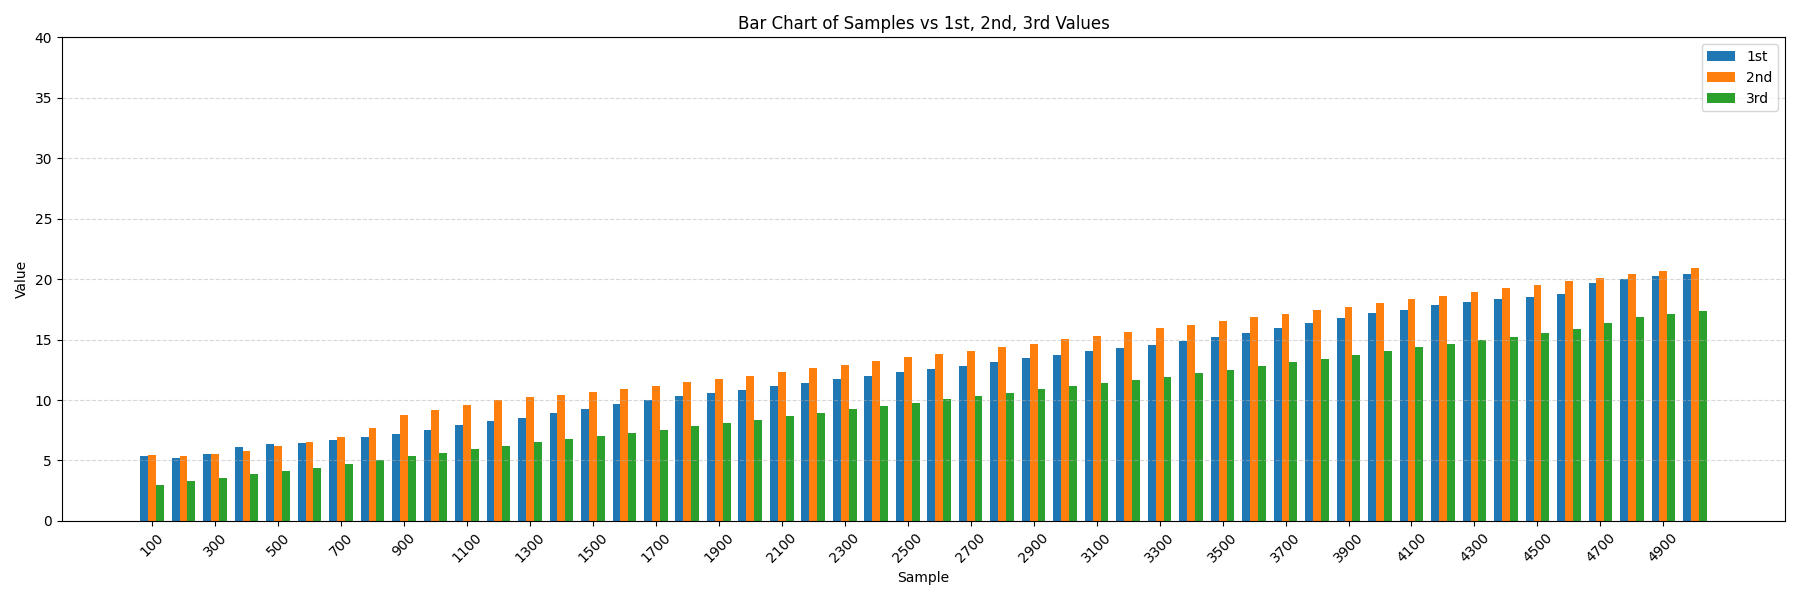
\includegraphics[width=0.8\linewidth]{gambar/Pembahasan/FIX_Render/render chart js_fix.png}
	\caption{Perbandingan Rendering Chart.js}
	\label{Perbandingan Rendering Chart.js}
\end{figure}

Hasil pengujian waktu render Chart.js pada tiga kali percobaan (1st, 2nd, dan 3rd) menunjukkan pola pertumbuhan yang konsisten seiring bertambahnya jumlah sampel data, dari 100 hingga 5000. Pada sampel terkecil, yaitu 100 data, waktu render pada percobaan pertama tercatat sebesar 5.36 ms, percobaan kedua 5.46 ms, dan percobaan ketiga 3.00 ms. Seiring bertambahnya jumlah data, tren kenaikan pada ketiga percobaan tampak serupa: misalnya pada 1000 data, waktu render untuk percobaan pertama naik menjadi 7.49 ms, percobaan kedua 9.19 ms, dan percobaan ketiga 5.65 ms. Pola yang sama terus berlanjut hingga data terbesar, yaitu 5000 sampel, di mana percobaan pertama mencapai 20.43 ms, percobaan kedua 20.91 ms, sedangkan percobaan ketiga tetap lebih rendah di angka 17.37 ms.

Data ini menunjukkan bahwa meskipun kondisi environment dan skrip yang digunakan sama, selalu muncul deviasi antar percobaan, terutama antara percobaan pertama dan kedua yang cenderung memiliki selisih mendekati stabil di rentang 0.5–1 ms, sedangkan percobaan ketiga relatif lebih cepat dengan selisih 2–3 ms lebih rendah dibanding dua percobaan lainnya. Fenomena ini mengindikasikan bahwa Chart.js mempertahankan konsistensi skalabilitas render di setiap percobaan meskipun ada variasi minor antar iterasi. Kenaikan waktu render mendekati linier sesuai penambahan beban data, yang wajar terjadi karena semakin banyak elemen visual dan kalkulasi yang harus diolah pada browser. Perbedaan antar percobaan kemungkinan besar berkaitan dengan variasi eksekusi di tingkat proses atau pengelolaan memori internal browser, meskipun secara teknis tidak ada perubahan pada sumber kode dan tidak dilakukan optimasi tambahan.

\subsection{D3}
Pengujian ini bertujuan untuk menilai kinerja D3 dalam menampilkan kemampuan rendering library D3 dengan volume data yang berbeda-beda. Proses pengukuran dimulai dari saat chart diinisialisasi hingga seluruh komponen visual sepenuhnya muncul di layar. Untuk memperoleh hasil yang konsisten, proses rendering dilakukan sebanyak tiga kali dengan D3.js. Berikut merupakan grafik perbandingan hasil dari ketiga percobaan tersebut:

\begin{table}[H]
	\centering
	\caption{Komparasi Render D3}
	\label{Komparasi Render D3}
	\renewcommand{\arraystretch}{1.2}
	\begin{tabular}{|c|c|c|c|}
		\hline
		\textbf{Samples} & \textbf{1\textsuperscript{st}} & \textbf{2\textsuperscript{nd}} & \textbf{3\textsuperscript{rd}} \\
		\hline
		100  & 0.35 & 0.58 & 0.40 \\
		200  & 0.62 & 1.05 & 0.79 \\
		300  & 0.59 & 1.50 & 1.13 \\
		400  & 0.60 & 2.03 & 1.66 \\
		500  & 0.73 & 1.81 & 2.03 \\
		600  & 0.93 & 1.72 & 2.39 \\
		700  & 1.26 & 1.80 & 2.77 \\
		\ldots & \ldots & \ldots & \ldots \\
		4400 & 14.91 & 15.69 & 17.38 \\
		4500 & 15.08 & 15.84 & 17.56 \\
		4600 & 15.25 & 15.99 & 17.72 \\
		4700 & 15.44 & 16.14 & 17.89 \\
		4800 & 15.81 & 16.31 & 18.06 \\
		4900 & 16.03 & 16.48 & 18.23 \\
		5000 & 16.23 & 16.66 & 18.41 \\
		\hline
	\end{tabular}
\end{table}

 	\begin{figure}[H]
	\centering
	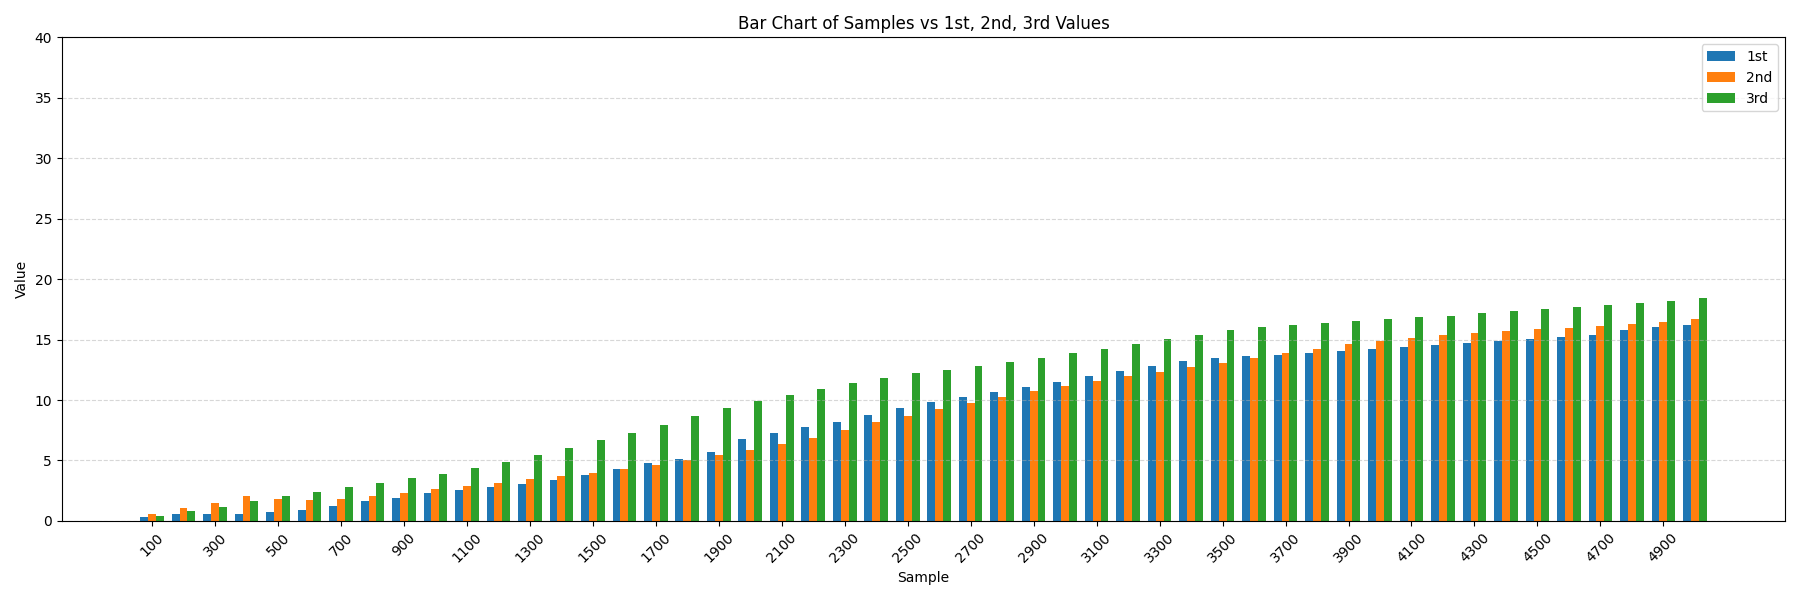
\includegraphics[width=0.8\linewidth]{gambar/Pembahasan/FIX_Render/d3.png}
	\caption{Perbandingan Rendering D3}
	\label{Perbandingan Rendering D3}
\end{figure}

Berdasarkan hasil pengamatan terhadap data rendering D3.js, ketiga percobaan memperlihatkan pola kenaikan waktu rendering yang konsisten seiring bertambahnya jumlah sampel data. Hal ini wajar mengingat D3.js memanfaatkan manipulasi DOM dan SVG secara intensif, sehingga makin banyak data yang dirender, makin besar pula beban prosesnya. 
Nilai pada percobaan pertama memperlihatkan pola pertumbuhan yang konsisten dan stabil, naik secara bertahap dari 0,35 ms hingga mencapai 16,20 di akhir rentang data, tanpa penurunan. Nilai percobaan kedua juga mengalami peningkatan yang stabil, bahkan lebih cepat dibandingkan pertama dalam beberapa titik data. Dimulai dari 0,58 ms, nilainya terus meningkat hingga menjadi yang tertinggi di titik akhir, yaitu 16,66ms. 
Nilai 3rd menunjukkan tren yang sedikit berbeda. Nilai ini tumbuh paling pesat dan mendominasi mencapai puncaknya di angka 18,41ms.
Meskipun masing-masing memiliki laju pertumbuhan yang berbeda dan pola yang sedikit bervariasi, terutama pada nilai percobaan ketiga yang sempat menurun di akhir, secara umum tren ketiganya tetap mengarah naik.


\subsection{highcharts}
Untuk menilai kemampuan render Highcharts dalam menampilkan berbagai jenis grafik dengan variasi jumlah data, dilakukan proses pengujian dengan mengukur waktu yang dibutuhkan sejak inisialisasi grafik hingga seluruh komponen visual sepenuhnya muncul di layar. Evaluasi ini dilakukan sebanyak tiga kali untuk menampilkan data dengan line chart, dan berikut merupakan hasil yang diperoleh dari penggunaan Highcharts dalam tiga eksperimen tersebut.

\begin{longtable}{|c|c|c|c|}
	\caption{\textit{Komparasi} Render Highcharts} \\
	\hline
	\textbf{Samples} & \textbf{1\textsuperscript{st}} & \textbf{2\textsuperscript{nd}} & \textbf{3\textsuperscript{rd}} \\
	\hline
	\endfirsthead
	\hline
	\textbf{Samples} & \textbf{1\textsuperscript{st}} & \textbf{2\textsuperscript{nd}} & \textbf{3\textsuperscript{rd}} \\
	\hline
	\endhead
100  & 34.35 & 38.80 & 24.57 \\
200  & 37.81 & 40.50 & 28.81 \\
300  & 38.37 & 41.77 & 29.50 \\
400  & 38.67 & 41.93 & 30.17 \\
500  & 38.55 & 41.27 & 30.40 \\
600  & 38.79 & 41.32 & 30.86 \\
700  & 38.53 & 41.20 & 31.26 \\
\ldots & \ldots & \ldots & \ldots \\
4400 & 40.91 & 41.68 & 37.20 \\
4500 & 41.06 & 41.77 & 37.44 \\
4600 & 41.22 & 41.89 & 37.73 \\
4700 & 41.40 & 41.99 & 37.98 \\
4800 & 41.52 & 42.10 & 38.44 \\
4900 & 41.64 & 42.21 & 39.17 \\
5000 & 41.82 & 42.35 & 39.95 \\
	\hline
\end{longtable}
 	\begin{figure}[H]
	\centering
	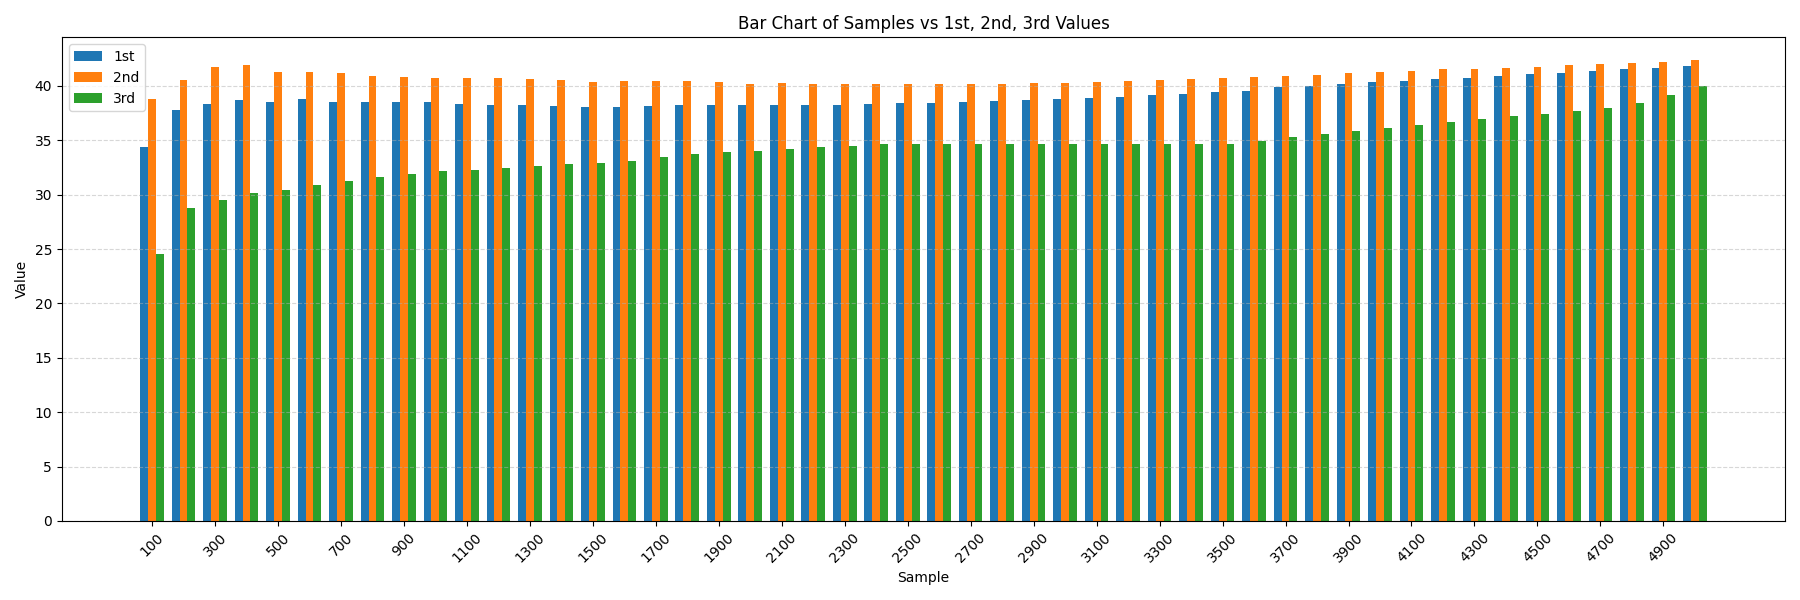
\includegraphics[width=0.8\linewidth]{gambar/Pembahasan/FIX_Render/hc.png}
	\caption{Perbandingan Rendering Highcharts}
	\label{Perbandingan Rendering Highcharts}
\end{figure}
Ditinjau dari ketiga eksperimen yang dilakukan, waktu render dengan library Highcharts meningkat di awal dan cenderung stabil di data dalam jumlah lebih dari 1000. Hal ini dikarenakan sebuah mekanisme TurboThreshold yang menjadi fitur default di dalam Highcharts yang belum berjalan. Fitur TurboThreshold ini adalah sebuah konfigurasi yang memungkinkan Highcharts untuk memvalidasi setiap titik yang dirender. Defaultnya, fitur ini akan mulai dijalankan secara otomatis saat jumlah data lebih dari 1000. Hal ini menjadi alasan yang valid karena setelah data ke 1000, tidak ada kenaikan waktu render yang signifikan dan kenaikan cenderung landai. 

\section{Pengukuran Penggunaan CPU}
Pengukuran penggunaan CPU ditinjau melalui Process ID (PID) terspesifik pada website. Fungsi dari pengukuraan CPU ini adalah untuk mengukur rata-rata penggunaan CPU saat digunakan untuk merender jumlah data tertentu. Tahapan yang dilakukan dalam pengukuran ini antara lain: 
\begin{enumerate}
	\item Membuka Task Manager pada Chrome untuk melihat PID dari tab yang digunakan. 
	\item Menuliskan PID pada kode yang telah dibuat. Kode ini berfungsi untuk mengambil nilai CPU yang digunakan pada suatu tab setiap detik. 
	 	\begin{figure}[H]
		\centering
		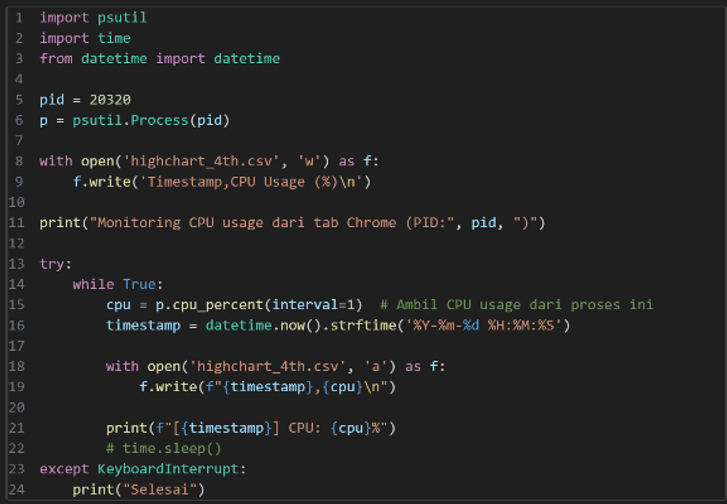
\includegraphics[width=0.8\linewidth]{gambar/Pembahasan/Mengukur CPU.png}
		\caption{Potongan Kode untuk Mengukur Penggunaan CPU}
		\label{Potongan Kode untuk Mengukur Penggunaan CPU}
	\end{figure}
	\item Nilai CPU tersebut kemudian akan disimpan dalam file csv.
\end{enumerate}


\subsection{Chart.js}
Pengukuran penggunaan CPU pada library Chart.js untuk menampilkan data IoT dalam bentuk line chart menunjukkan hasil seperti berikut : 
\begin{longtable}{|c|c|c|c|}
	\caption{Komparasi CPU \textit{Chart.js}} \\
	\hline
	\textbf{Samples} & \textbf{1\textsuperscript{st}} & \textbf{2\textsuperscript{nd}} & \textbf{3\textsuperscript{rd}} \\
	\hline
	\endfirsthead
	\hline
	\textbf{Samples} & \textbf{1\textsuperscript{st}} & \textbf{2\textsuperscript{nd}} & \textbf{3\textsuperscript{rd}} \\
	\hline
	\endhead
	100  & 0.22 & 0.18 & 0.15 \\
	200  & 0.21 & 0.19 & 0.13 \\
	300  & 0.25 & 0.19 & 0.13 \\
	400  & 0.23 & 0.20 & 0.14 \\
	500  & 0.24 & 0.21 & 0.14 \\
	600  & 0.24 & 0.22 & 0.15 \\
	700  & 0.25 & 0.23 & 0.16 \\
	\ldots & \ldots & \ldots & \ldots \\
	4400 & 0.85 & 0.68 & 0.53 \\
	4500 & 0.86 & 0.69 & 0.55 \\
	4600 & 0.87 & 0.70 & 0.56 \\
	4700 & 0.86 & 0.71 & 0.56 \\
	4800 & 0.85 & 0.72 & 0.55 \\
	4900 & 0.86 & 0.73 & 0.54 \\
	5000 & 0.86 & 0.74 & 0.54 \\
	\hline
\end{longtable}

	\begin{figure}[H]
	\centering
	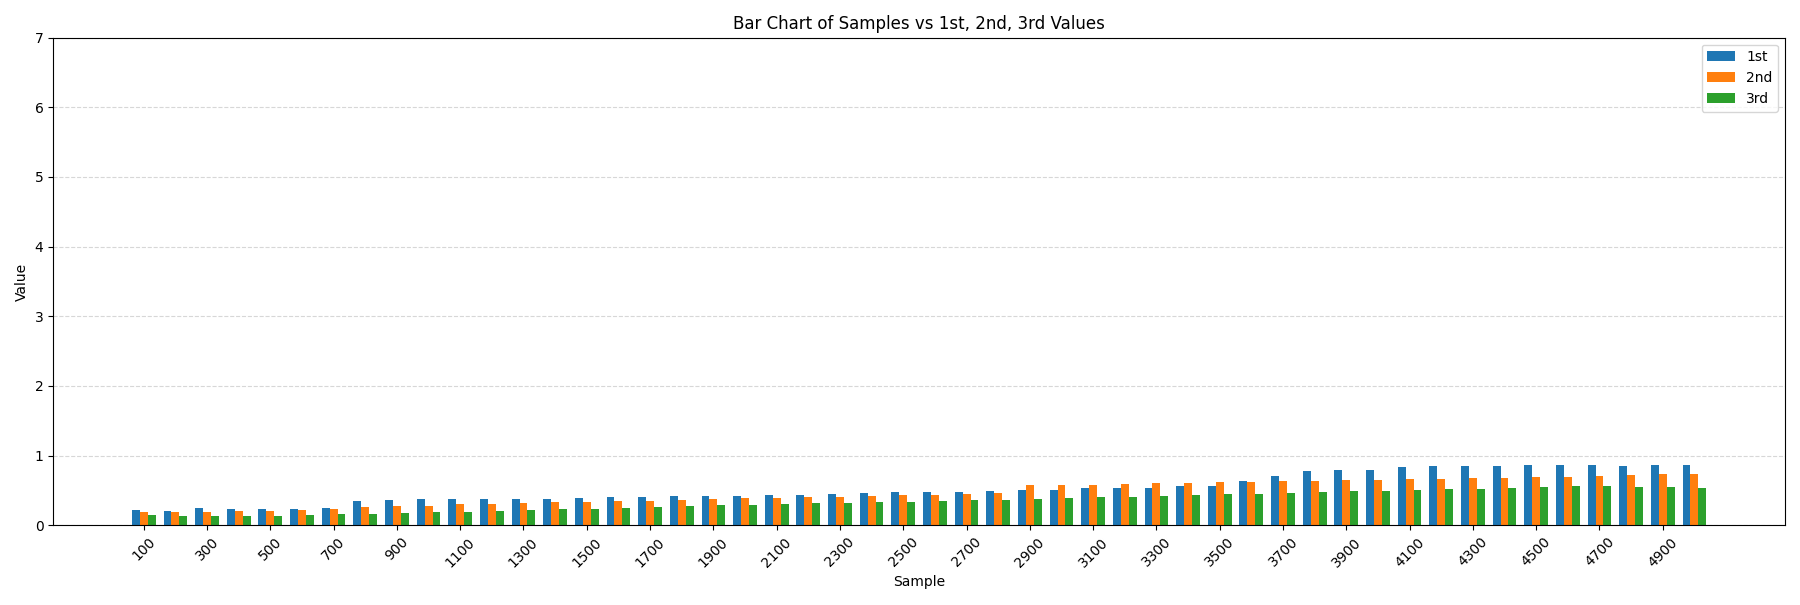
\includegraphics[width=0.8\linewidth]{gambar/Pembahasan/FIX_CPU/cjs compare.png}
	\caption{Grafik Komparasi Chart.js}
	\label{Grafik Komparasi Chart.js}
\end{figure}

Dari ketiga eksperimen yang dilakukan, penggunaan CPU pada library Chart.js untuk menampilkan data IoT memiliki kemiripan. Grafik kenaikan di semua iterasi pun terlihat landai. Hal ini dikarenakan Chart.js menggunakan canvas rendering yang lebih menggunakan resource GPU disbanding CPU.
Dari grafik tersebut, eksperimen kedua menunjukkan peningkatan penggunaan CPU setelah 2900 data. Hal ini dapat mengindikasikan terjadi lonjakan di waktu render dan/atau penggunaan memori. Meskipun begitu, ketiganya konsisten menunjukkan kenaikan penggunaan CPU seiring bertambahnya jumlah data.

\subsection{D3}
Pengukuran penggunaan CPU pada library D3 untuk menampilkan data IoT dalam bentuk line chart menunjukkan hasil seperti berikut : 
\begin{longtable}{|c|c|c|c|}
	\caption{Komparasi CPU \textit{Chart.js}} \\
	\hline
	\textbf{Samples} & \textbf{1\textsuperscript{st}} & \textbf{2\textsuperscript{nd}} & \textbf{3\textsuperscript{rd}} \\
	\hline
	\endfirsthead
	\hline
100  & 0.20 & 0.46 & 0.22 \\
200  & 0.16 & 0.53 & 0.28 \\
300  & 0.14 & 0.64 & 0.35 \\
400  & 0.13 & 0.77 & 0.46 \\
500  & 0.14 & 0.91 & 0.61 \\
600  & 0.16 & 1.03 & 0.74 \\
700  & 0.19 & 1.14 & 0.86 \\
\ldots & \ldots & \ldots & \ldots \\
4400 & 5.10 & 5.56 & 5.64 \\
4500 & 5.21 & 5.46 & 5.75 \\
4600 & 5.33 & 5.36 & 5.74 \\
4700 & 5.45 & 5.44 & 5.73 \\
4800 & 5.57 & 5.57 & 5.73 \\
4900 & 5.70 & 5.71 & 5.74 \\
5000 & 5.83 & 5.84 & 5.76 \\
	\hline
\end{longtable}

	\begin{figure}[H]
	\centering
	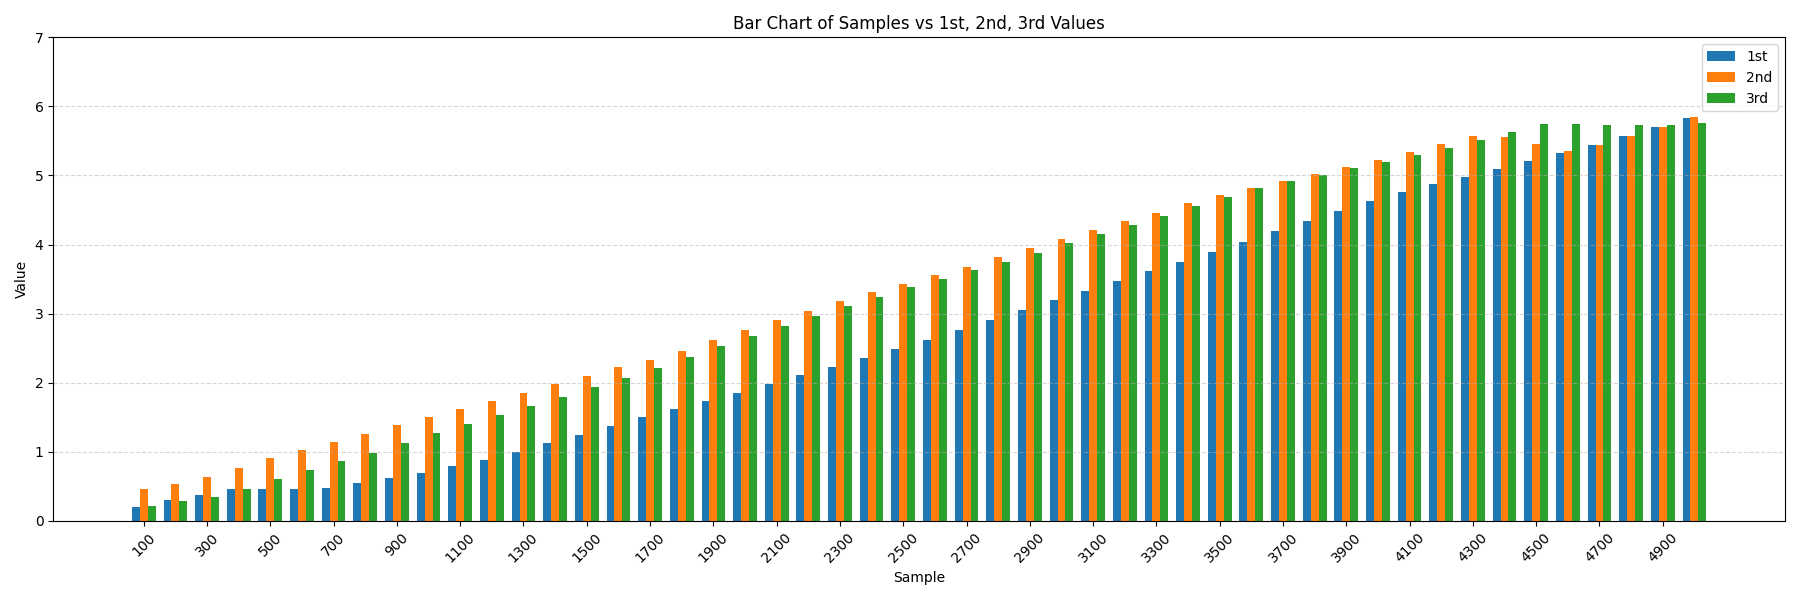
\includegraphics[width=0.8\linewidth]{gambar/Pembahasan/FIX_CPU/d3_compare.png}
	\caption{Grafik Komparasi D3}
	\label{Grafik Komparasi D3}
\end{figure}
Ketiga grafik memiliki pola kenaikan yang sama karena peningkatan ukuran data, peningkatan render elemen DOM, dan rendering grafik yang semakin kompleks. Kenaikan CPU pada proses ini mencapai titik tertinggi di 5,8 ms dan tren ini terjadi pada ketiga eksperimen yang dilakukan. 

\subsection{Highcharts}
Pengukuran penggunaan CPU pada library Highcharts untuk menampilkan data IoT dalam bentuk line chart menunjukkan hasil seperti berikut : 
\begin{table}[H]
	\centering
	\caption{Komparasi CPU pada \textit{Highcharts}}
	\begin{tabular}{|c|c|c|c|}
		\hline
		\textbf{Samples} & \textbf{1\textsuperscript{st}} & \textbf{2\textsuperscript{nd}} & \textbf{3\textsuperscript{rd}} \\
		\hline
		100  & 2.28 & 4.30 & 2.83 \\
		200  & 3.84 & 4.22 & 2.79 \\
		300  & 3.92 & 4.13 & 2.86 \\
		400  & 4.31 & 4.43 & 2.89 \\
		500  & 4.78 & 4.76 & 2.97 \\
		600  & 5.09 & 5.10 & 3.04 \\
		700  & 5.40 & 5.39 & 3.13 \\
		\ldots & \ldots & \ldots & \ldots \\
		4400 & 6.00 & 6.77 & 5.13 \\
		4500 & 5.88 & 6.78 & 5.16 \\
		4600 & 5.76 & 6.80 & 5.19 \\
		4700 & 5.65 & 6.81 & 5.14 \\
		4800 & 5.54 & 6.82 & 5.04 \\
		4900 & 5.44 & 6.83 & 4.94 \\
		5000 & 5.34 & 6.84 & 4.85 \\
		\hline
	\end{tabular}
\end{table}

	\begin{figure}[H]
	\centering
	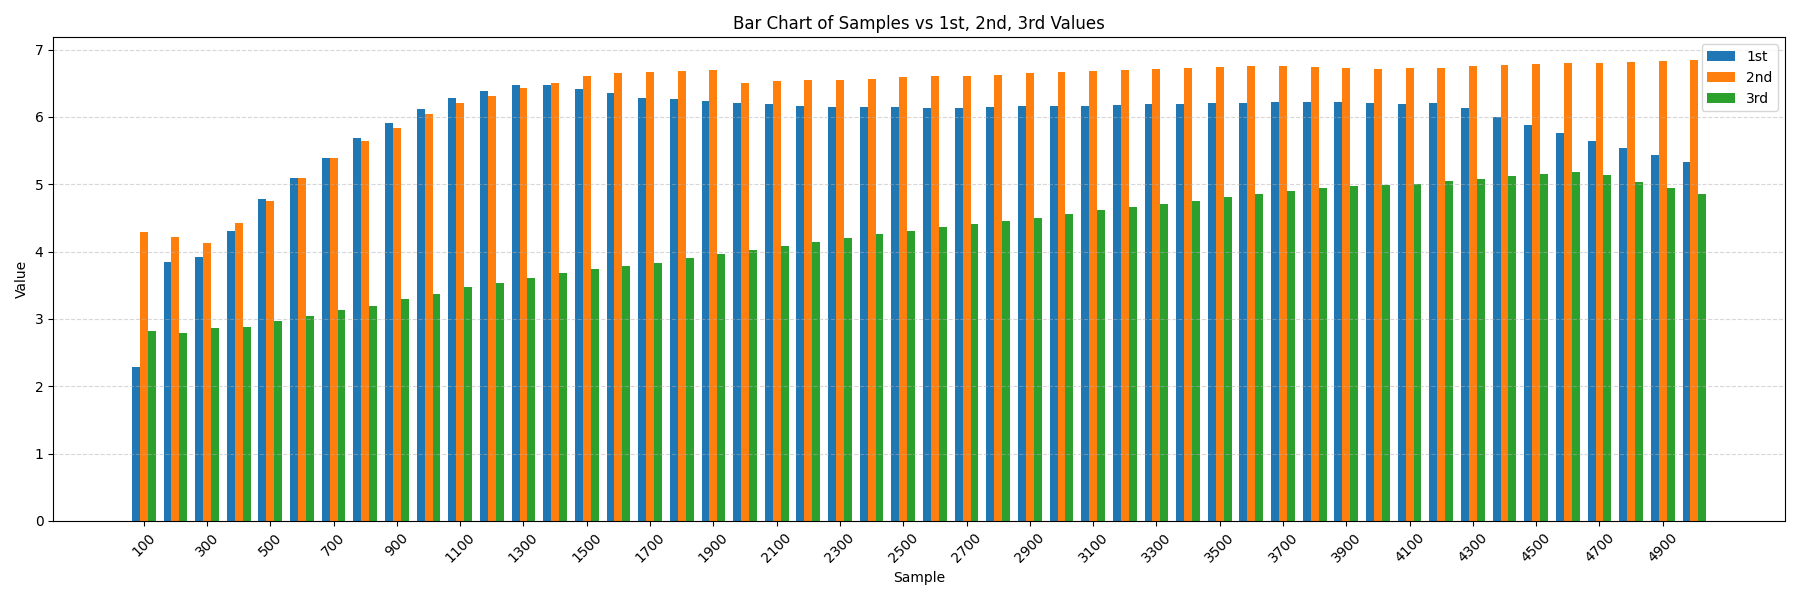
\includegraphics[width=0.8\linewidth]{gambar/Pembahasan/FIX_CPU/hc_compare.png}
	\caption{Grafik Komparasi Highcharts}
	\label{Grafik Komparasi Highcharts}
\end{figure}

Dari ketiga eksperimen yang dilakukan, secara konsisten terdapat peningkatan penggunaan CPU saat data kurang dari 1500 kemudian setelahnya data menjadi lebih stabil atau mengalami penurunan. Hal ini dapat disebabkan oleh fungsi TurboThreshold yang juga turut mempengaruhi performa render dan penggunaan memori. 


\section{Pengukuran Footprint Memory}
Pengukuran penggunaan memori dintinjau dari penggunaan footprint memory pada sebuah halaman website spesifik yang mengukur private memory, heap memory untuk menyimpan objek di dalam website termasuk data dari json yang ditampilkan, dan stack memory untuk menyimpan variabel lokal dan kontrol eksekusi fungsi. Langkah yang dilakukan pada tahap ini adalah sebagai berikut :

\begin{enumerate}
\item Menampilkan visualisasi pada tab incognito 
\item Meninjau penggunaan memory footprint yang dapat diakses melalui Task Manager pada Chrome
\item Mencatat performa di tiap titik yang telah ditentukan, yaitu 100, 200, 300, 400, dan seterusnya hingga data ke 5000
Langkah tersebut dilakukan sebanyak tiga kali eksperimen di tiap-tiap library untuk mengukur penggunaan memorinya.  
\end{enumerate} 
\subsection{Chart.js}
Pengukuran memori pada Chart.js dalam tiga eksperimen menghasilkan grafik perbandingan seperti berikut :
\begin{table}[H]
	\centering
	\caption{Komparasi Memori \textit{Chart.js}}
	\begin{tabular}{|c|c|c|c|}
		\hline
		\textbf{Samples} & \textbf{1\textsuperscript{st}} & \textbf{2\textsuperscript{nd}} & \textbf{3\textsuperscript{rd}} \\
		\hline
		100  & 56{,}730 & 59{,}600  & 56{,}883 \\
		200  & 57{,}460 & 66{,}959  & 58{,}921 \\
		300  & 66{,}104 & 74{,}317  & 60{,}734 \\
		400  & 70{,}215 & 81{,}676  & 62{,}489 \\
		500  & 74{,}326 & 89{,}035  & 64{,}120 \\
		600  & 78{,}437 & 96{,}394  & 65{,}871 \\
		700  & 82{,}548 & 103{,}752 & 67{,}534 \\
		\ldots & \ldots & \ldots & \ldots \\
		4400 & 152{,}967 & 142{,}615 & 146{,}051 \\
		4500 & 155{,}905 & 143{,}490 & 146{,}128 \\
		4600 & 157{,}111 & 144{,}365 & 146{,}152 \\
		4700 & 154{,}744 & 145{,}240 & 146{,}062 \\
		4800 & 156{,}783 & 148{,}564 & 146{,}067 \\
		4900 & 155{,}316 & 151{,}889 & 146{,}070 \\
		5000 & 154{,}872 & 155{,}213 & 146{,}072 \\
		\hline
	\end{tabular}
\end{table}

	\begin{figure}[H]
	\centering
	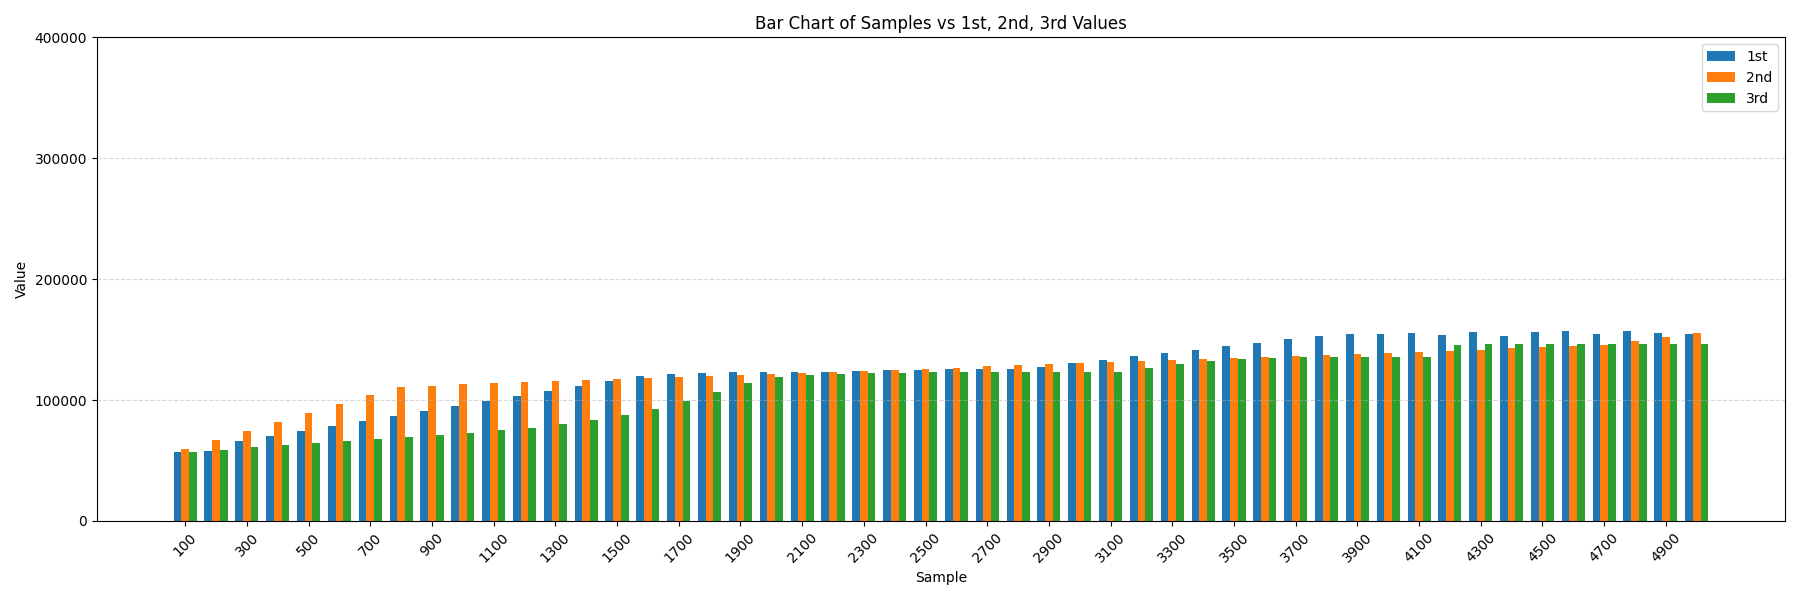
\includegraphics[width=0.8\linewidth]{gambar/Pembahasan/FIX_Memori/cjs.png}
	\caption{Grafik Komparasi Chart.js}
	\label{Grafik Komparasi Chart.js}
\end{figure}


Dari ketiga eksperimen yang tertampil pada grafik, dapat diamati bahwa proses rendering menggunakan library Chart.js menunjukan peningkatan konsumsi footprint memory yang bertahap di setiap pertambahan jumlah data. Hal ini menunjukkan adanya akumulasi beban render pada tiap eksperimen yang disebabkan oleh peningkatan kompleksitas visualisasi dan jumlah elemen yang dirender ulang untuk menampilkan data dengan jumlah data yang selalu meningkat. 

\subsection{D3}
Pengukuran memori pada D3 dalam tiga eksperimen menghasilkan grafik perbandingan seperti berikut :
\begin{table}[H]
	\centering
	\caption{Komparasi Memori \textit{D3.js}}
	\begin{tabular}{|c|c|c|c|}
		\hline
		\textbf{Samples} & \textbf{1\textsuperscript{st}} & \textbf{2\textsuperscript{nd}} & \textbf{3\textsuperscript{rd}} \\
		\hline
		100  & 108{,}144 &  52{,}290 & 108{,}203 \\
		200  & 112{,}211 &  60{,}310 & 112{,}289 \\
		300  & 120{,}125 &  68{,}940 & 120{,}145 \\
		400  & 128{,}039 &  77{,}520 & 128{,}070 \\
		500  & 135{,}953 &  86{,}380 & 136{,}005 \\
		600  & 143{,}883 &  95{,}670 & 143{,}920 \\
		700  & 161{,}812 & 105{,}290 & 161{,}850 \\
		\ldots & \ldots & \ldots & \ldots \\
		4400 & 498{,}702 & 494{,}992 & 511{,}000 \\
		4500 & 499{,}774 & 473{,}502 & 515{,}200 \\
		4600 & 500{,}344 & 473{,}790 & 518{,}000 \\
		4700 & 500{,}812 & 474{,}080 & 519{,}000 \\
		4800 & 501{,}496 & 487{,}760 & 519{,}600 \\
		4900 & 501{,}855 & 494{,}600 & 519{,}900 \\
		5000 & 502{,}214 & 501{,}440 & 520{,}120 \\
		\hline
	\end{tabular}
\end{table}
	\begin{figure}[H]
	\centering
	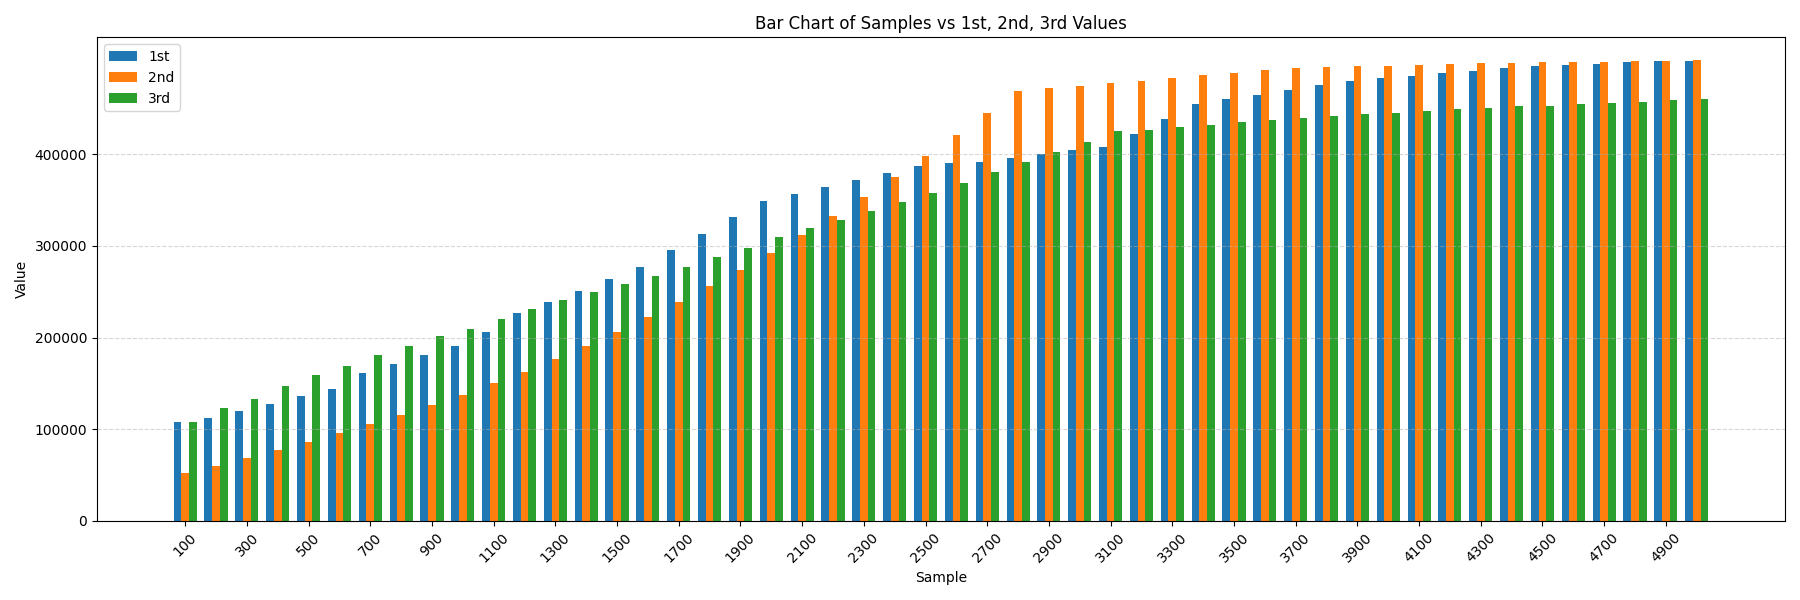
\includegraphics[width=0.8\linewidth]{gambar/Pembahasan/FIX_Memori/D3.png}
	\caption{Grafik Komparasi D3}
	\label{Grafik Komparasi D3}
\end{figure}

Terdapat selisih yang cukup besar pada eksperimen ketiga jika dibandingkan dengan eksperimen 1 dan eksperimen 2. Hal ini mengindikasikan terdapat kemungkinan DOM yang tidak dibersihkan. Namun, ditinjau dari tren dan hasil pengukuran dua eksperimen lainnya, pola tren penggunaan memori dari ketiga eksperimen tetap menunjukkan konsistensi. Ketiganya mencerminkan peningkatan footprint memory secara bertahap seiring bertambahnya jumlah data yang di-render. Hal ini menjelaskan bahwa D3.js secara umum menunjukkan karakteristik peningkatan konsumsi memori yang linier terhadap pertambahan kompleksitas dan jumlah data yang divisualisasikan.

\subsection{Highcharts}
Pengukuran memori pada Highcharts dalam tiga kali eksperimen menunjukkan hasil  seperti berikut :
\begin{table}[H]
	\centering
	\caption{Komparasi Memori \textit{Highcharts}}
	\begin{tabular}{|c|c|c|c|}
		\hline
		\textbf{Samples} & \textbf{1\textsuperscript{st}} & \textbf{2\textsuperscript{nd}} & \textbf{3\textsuperscript{rd}} \\
		\hline
		100  & 97,183   & 70,350   & 83,214   \\
		200  & 106,565  & 92,120   & 91,500   \\
		300  & 111,724  & 108,760  & 100,200  \\
		400  & 113,001  & 131,100  & 108,600  \\
		500  & 116,409  & 143,870  & 117,800  \\
		600  & 126,316  & 150,550  & 124,300  \\
		700  & 132,553  & 157,700  & 130,800  \\
		\ldots & \ldots & \ldots & \ldots \\
		4400 & 335,295  & 404,300  & 386,200  \\
		4500 & 338,330  & 407,250  & 388,000  \\
		4600 & 350,158  & 410,600  & 390,200  \\
		4700 & 358,557  & 414,200  & 420,268  \\
		4800 & 365,698  & 417,800  & 390,084  \\
		4900 & 369,709  & 418,450  & 381,600  \\
		5000 & 398,125  & 420,510  & 383,616  \\
		\hline
	\end{tabular}
\end{table}

	\begin{figure}[H]
	\centering
	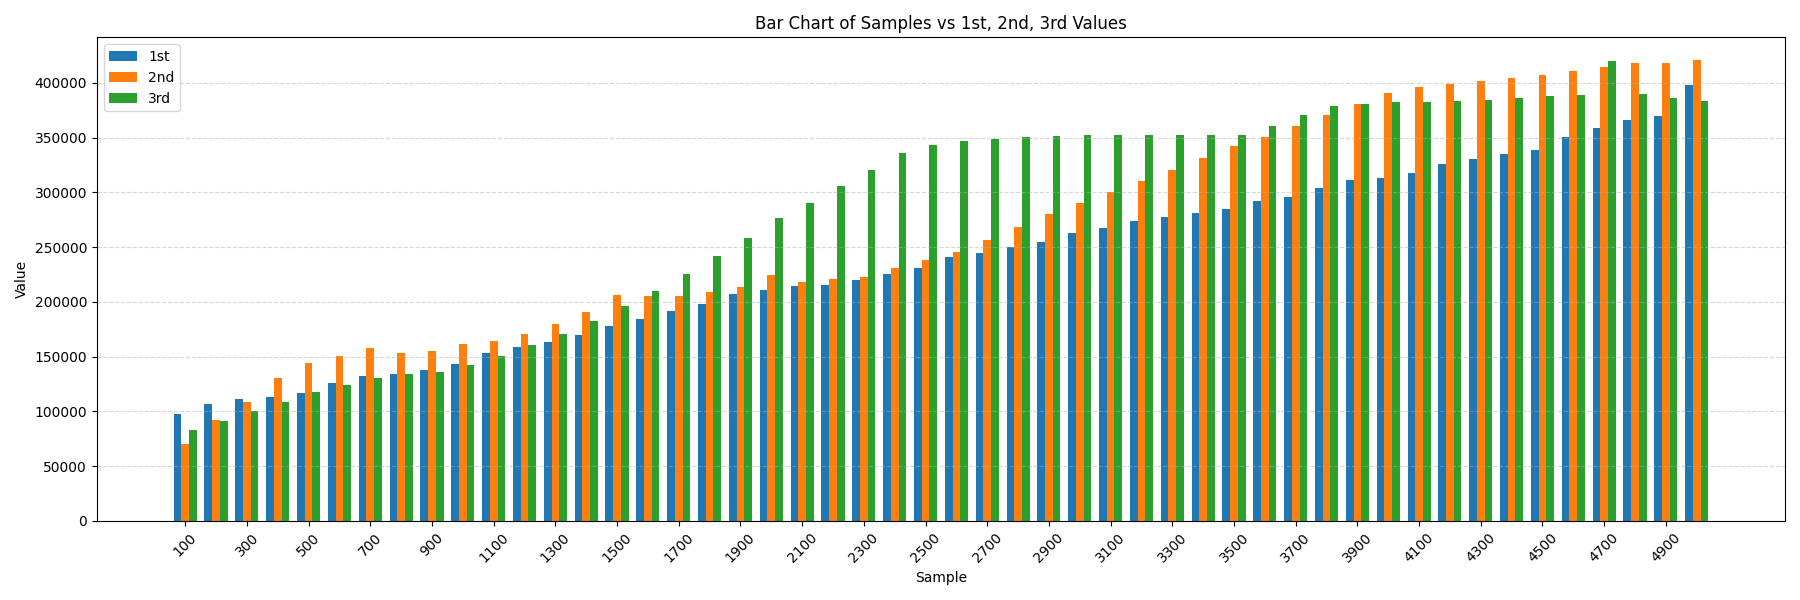
\includegraphics[width=0.8\linewidth]{gambar/Pembahasan/FIX_Memori/hc.png}
	\caption{Grafik Komparasi Highcharts}
	\label{Grafik Komparasi Highcharts}
\end{figure}

Grafik yang ditampilkan menunjukkan perbandingan penggunaan memori dari \textit{library} Highcharts selama proses pengujian berulang, dengan kondisi lingkungan dan kode yang digunakan sama persis untuk ketiga skenario. Karena variabel-variabel eksternal dikendalikan secara ketat, perbedaan konsumsi memori yang muncul kemungkinan besar disebabkan oleh perilaku internal Highcharts saat runtime, seperti mekanisme Highcharts dalam mengelola objek grafik, menyimpan cache, atau menjalankan proses pembaruan visual.
Pada pengujian pertama, terlihat pola kenaikan memori yang cenderung stabil dan terukur. Hal ini mengindikasikan bahwa proses pembersihan memori atau pengelolaan ulang elemen-elemen grafik berjalan cukup baik. Sebaliknya, pada pengujian kedua, lonjakan memori terjadi cukup drastis saat jumlah eksperimen bertambah. Hal ini mengarah pada kemungkinan terjadinya penumpukan elemen atau data yang tidak segera dibersihkan, Sementara itu, hasil pengujian ketiga memperlihatkan lonjakan penggunaan memori yang cukup cepat di awal, tetapi kemudian stagnan di pertengahan grafik. Hal ini menunjukkan bahwa pada titik tertentu, Highcharts mulai membatasi pemrosesan atau secara otomatis melakukan optimasi agar konsumsi memori tidak terus naik. Namun, di bagian akhir grafik, nilainya kembali naik atau justru menurun, yang bisa mengindikasikan adanya proses pembersihan memori oleh sistem.

\section{Analisis Skalabilitas}
Analisis dan komparasi digunakan untuk membandingkan setiap library dan pengaruhnya terhadap parameter-parameter yang diukur dengan kuantitas data tertentu dalam jumlah yang sama pada lingkungan dan kondisi yang seragam. Pengujian dilakukan secara berulang guna memperoleh nilai yang representatif. Hasil dari perbandingan tersebut ditampilkan dalam bentuk grafik

\subsection{Performa Rendering}
Analisis performa rendering dilakukan dalam tiga kali eksperimen untuk mengevaluasi efisiensi masing-masing library visualisasi data, yakni Chart.js, D3.js, dan Highcharts dengan hasil seperti berikut
\begin{table}[H]
	\centering
	\caption{Komparasi Rendering Library Chart.js, D3.js, dan Highcharts}
	\begin{tabular}{|c|ccc|ccc|ccc|}
		\hline
		\textbf{Sample} & \multicolumn{3}{c|}{\textbf{Chart.js}} & \multicolumn{3}{c|}{\textbf{D3.js}} & \multicolumn{3}{c|}{\textbf{Highcharts}} \\
		& \textbf{1\textsuperscript{st}} & \textbf{2\textsuperscript{nd}} & \textbf{3\textsuperscript{rd}} & \textbf{1\textsuperscript{st}} & \textbf{2\textsuperscript{nd}} & \textbf{3\textsuperscript{rd}} & \textbf{1\textsuperscript{st}} & \textbf{2\textsuperscript{nd}} & \textbf{3\textsuperscript{rd}} \\
		\hline
		100  & 5.36 & 5.46 & 3.00 & 0.35 & 0.58 & 0.40 & 34.35 & 38.80 & 24.57 \\
		200  & 5.19 & 5.35 & 3.27 & 0.62 & 1.05 & 0.79 & 37.81 & 40.50 & 28.81 \\
		300  & 5.56 & 5.54 & 3.58 & 0.59 & 1.50 & 1.13 & 38.37 & 41.77 & 29.50 \\
		400  & 6.10 & 5.77 & 3.86 & 0.60 & 2.03 & 1.66 & 38.67 & 41.93 & 30.17 \\
		500  & 6.40 & 6.20 & 4.13 & 0.73 & 1.81 & 2.03 & 38.55 & 41.27 & 30.40 \\
		600  & 6.42 & 6.50 & 4.41 & 0.93 & 1.72 & 2.39 & 38.79 & 41.32 & 30.86 \\
		700  & 6.66 & 6.92 & 4.72 & 1.26 & 1.80 & 2.77 & 38.53 & 41.20 & 31.26 \\
		\ldots & \ldots & \ldots & \ldots & \ldots & \ldots & \ldots & \ldots & \ldots & \ldots \\
		4400 & 18.33 & 19.23 & 15.25 & 14.91 & 15.69 & 17.38 & 40.91 & 41.68 & 37.20 \\
		4500 & 18.55 & 19.51 & 15.55 & 15.08 & 15.84 & 17.56 & 41.06 & 41.77 & 37.44 \\
		4600 & 18.78 & 19.81 & 15.86 & 15.25 & 15.99 & 17.72 & 41.22 & 41.89 & 37.73 \\
		4700 & 19.72 & 20.10 & 16.40 & 15.44 & 16.14 & 17.89 & 41.40 & 41.99 & 37.98 \\
		4800 & 20.02 & 20.44 & 16.87 & 15.81 & 16.31 & 18.06 & 41.52 & 42.10 & 38.44 \\
		4900 & 20.23 & 20.66 & 17.12 & 16.03 & 16.48 & 18.23 & 41.64 & 42.21 & 39.17 \\
		5000 & 20.43 & 20.91 & 17.37 & 16.23 & 16.66 & 18.41 & 41.82 & 42.35 & 39.95 \\
		\hline
	\end{tabular}
\end{table}

	\begin{figure}[H]
	\centering
	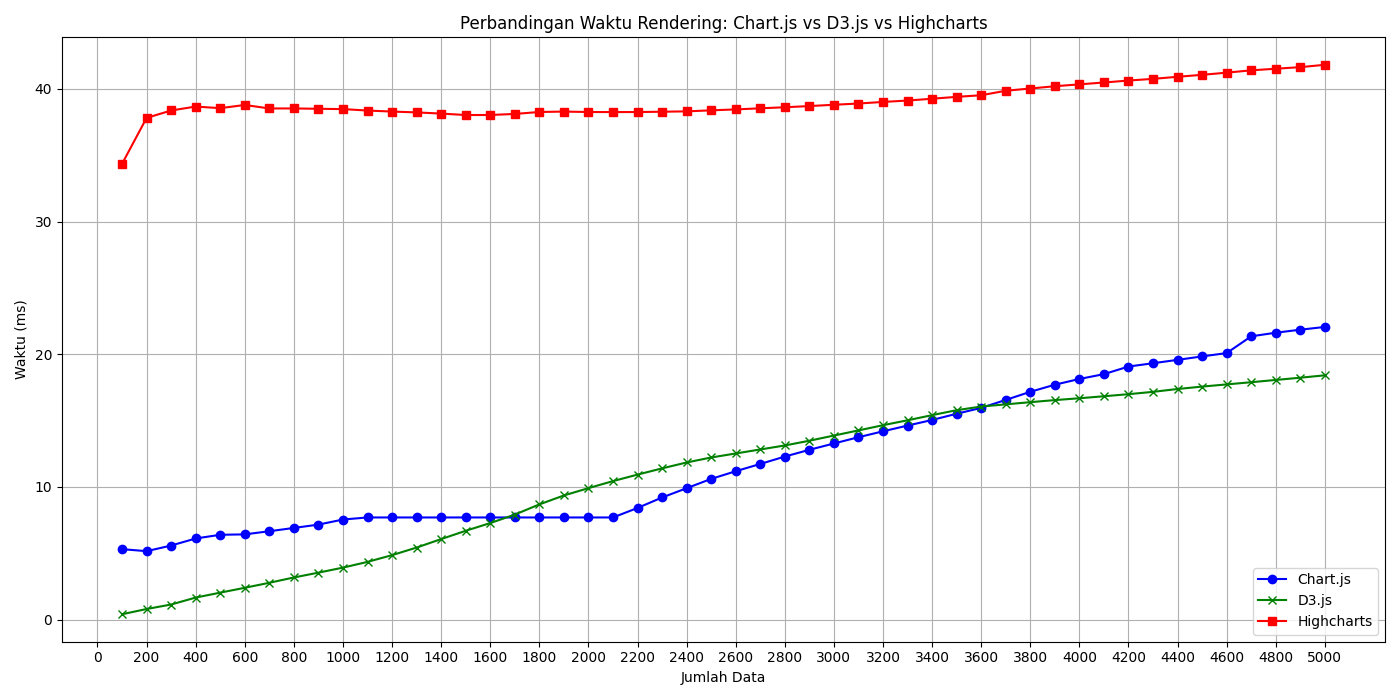
\includegraphics[width=0.8\linewidth]{gambar/Pembahasan/FIX_Render/Figure_1.png}
	\caption{Grafik Komparasi Render Pertama}
	\label{Grafik Komparasi Render Pertama}
\end{figure}

Pada eksperimen pertama, ditemukan perbedaan yang cukup mencolok antara Chart.js, D3.js, dan Highcharts dalam hal kecepatan rendering. 

Meskipun Chart.js dan D3 masih dapat bersaing dengan performa yang cukup baik, Chart.js menunjukkan waktu render yang lebih konsisten meskipun lebih tinggi dibanding D3. Sementara itu, Highcharts memiliki waktu render yang paling tinggi. Saat jumlah data meningkat hingga mencapai 5000 entri, baik Chart.js maupun D3.js masih mampu merespon dengan waktu rendering yang relatif stabil dan tidak menunjukkan lonjakan performa yang drastis. Hal ini menunjukkan bahwa keduanya cukup andal untuk penggunaan dengan skala data menengah. Selain itu, Highcharts juga menunjukkan penurunan waktu render dan lebih stabil setelah melewati ambang 1000 data. Penurunan ini disebabkan oleh fitur turbo threshold bawaan Highcharts yang secara otomatis membatasi kompleksitas rendering demi menjaga kestabilan. 

Pada eksperimen kedua, ketiga library menunjukkan tren yang sama. Dari grafik tersebut, terlihat bahwa D3 memiliki performa terbaik secara konsisten diikuti oleh Chart.js dan Highcharts yang cenderung konstan namun memiliki waktu render yang cukup tinggi.

	\begin{figure}[H]
	\centering
	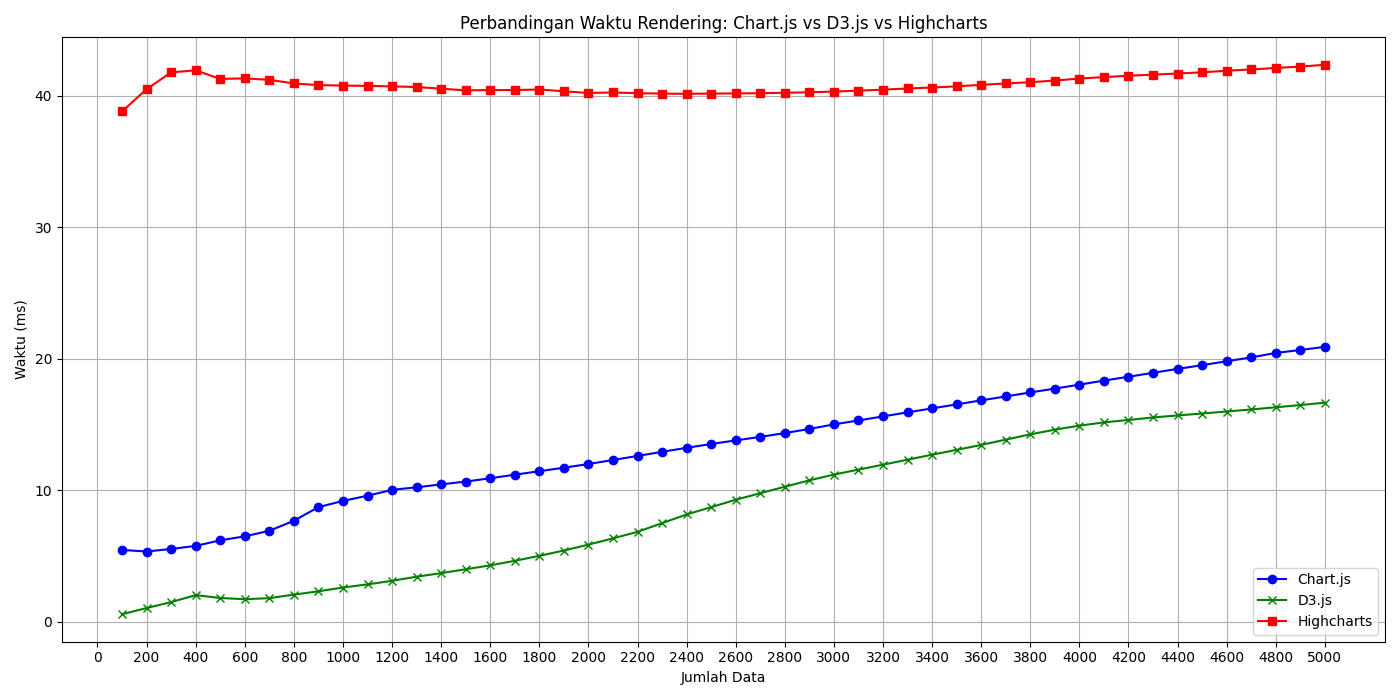
\includegraphics[width=0.8\linewidth]{gambar/Pembahasan/FIX_Render/Figure_2.png}
	\caption{Grafik Komparasi Render Kedua}
	\label{Grafik Komparasi Render Kedua}
\end{figure}
D3.js menunjukkan peningkatan waktu eksekusi yang linear namun tetap paling rendah dibandingkan dua library lainnya. Chart.js juga menunjukkan peningkatan linear yang tidak berbeda jauh dengan D3. Kedua library ini mengalami peningkatan di setiap kenaikan jumlah data dengan selisih waktu render kurang dari 5ms. Sementara itu, Highcharts menunjukkan karakteristik rendering seperti pada eksperimen pertama. Highcharts memiliki waktu rendering yang cukup lama dan mengalami peningkatan namun cenderung konstan setelah jumlah data lebih dari 1000.

Pada eksperimen ketiga, terdapat beberapa perbedaan dari eksperimen sebelumnya. Pada eksperimen ini, D3 memiliki waktu render yang lebih tinggi dari Chart.js pada titik 3400 hingga 4600 dengan selisih data tidak lebih dari 1ms. 
	\begin{figure}[H]
	\centering
	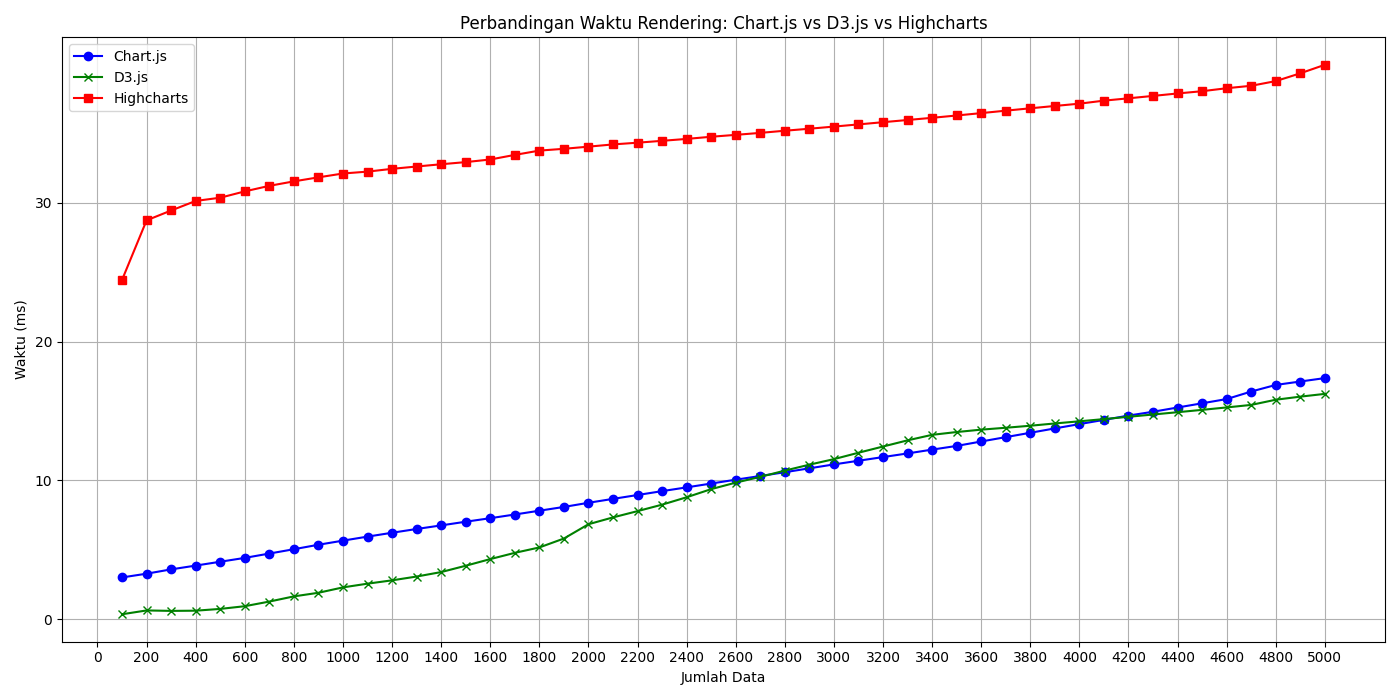
\includegraphics[width=0.8\linewidth]{gambar/Pembahasan/FIX_Render/Figure_3.png}
	\caption{Grafik Komparasi Render ketiga}
	\label{Grafik Komparasi Render Ketiga}
\end{figure}
Namun, secara keseluruhan, pola tren pada eksperimen ini serupa dengan eksperimen sebelumnya yang menunjukkan D3 masih menjadi library dengan waktu render paling rendah. 

\subsection{Alokasi CPU}
Analisis alokasi CPU dilakukan dalam tiga kali eksperimen untuk mengevaluasi efisiensi masing-masing library visualisasi data, yakni Chart.js, D3.js, dan Highcharts.
\begin{table}[H]
	\centering
	\caption{Komparasi Penggunaan CPU}
	\begin{tabular}{|c|ccc|ccc|ccc|}
		\hline
		\textbf{Sample} & \multicolumn{3}{c|}{\textbf{Chart.js}} & \multicolumn{3}{c|}{\textbf{D3.js}} & \multicolumn{3}{c|}{\textbf{Highcharts}} \\
		& \textbf{1\textsuperscript{st}} & \textbf{2\textsuperscript{nd}} & \textbf{3\textsuperscript{rd}} & \textbf{1\textsuperscript{st}} & \textbf{2\textsuperscript{nd}} & \textbf{3\textsuperscript{rd}} & \textbf{1\textsuperscript{st}} & \textbf{2\textsuperscript{nd}} & \textbf{3\textsuperscript{rd}} \\
		\hline
		100  & 0.22 & 0.18 & 0.15 & 0.22 & 0.46 & 0.20 & 2.28 & 4.30 & 2.83 \\
		200  & 0.20 & 0.19 & 0.13 & 0.28 & 0.50 & 0.36 & 1.84 & 4.22 & 2.32 \\
		300  & 0.25 & 0.19 & 0.13 & 0.28 & 0.53 & 0.19 & 2.28 & 4.42 & 2.89 \\
		400  & 0.24 & 0.23 & 0.14 & 0.26 & 0.64 & 0.26 & 2.42 & 4.44 & 3.00 \\
		500  & 0.24 & 0.21 & 0.14 & 0.29 & 0.65 & 0.28 & 1.78 & 4.76 & 2.97 \\
		600  & 0.24 & 0.23 & 0.16 & 0.30 & 0.72 & 0.40 & 1.94 & 5.06 & 3.27 \\
		700  & 0.25 & 0.22 & 0.15 & 0.34 & 0.80 & 0.49 & 2.10 & 5.39 & 3.13 \\
		\ldots & \ldots & \ldots & \ldots & \ldots & \ldots & \ldots & \ldots & \ldots & \ldots \\
		4400 & 0.85 & 0.68 & 0.53 & 5.64 & 5.60 & 5.10 & 6.77 & 5.13 & 4.93 \\
		4500 & 0.86 & 0.69 & 0.56 & 5.75 & 5.36 & 5.14 & 5.88 & 6.80 & 5.15 \\
		4600 & 0.87 & 0.70 & 0.56 & 5.74 & 5.36 & 5.33 & 5.76 & 6.80 & 5.19 \\
		4700 & 0.86 & 0.71 & 0.56 & 5.73 & 5.44 & 5.45 & 6.55 & 6.81 & 5.14 \\
		4800 & 0.85 & 0.72 & 0.54 & 5.73 & 5.57 & 5.54 & 6.34 & 6.94 & 4.85 \\
		4900 & 0.86 & 0.73 & 0.54 & 5.74 & 5.70 & 5.54 & 6.34 & 6.84 & 4.93 \\
		5000 & 0.86 & 0.74 & 0.54 & 5.76 & 5.84 & 5.33 & 6.34 & 6.84 & 4.85 \\
		\hline
	\end{tabular}
\end{table}
Pada eksperimen pertama, Chart.js menunjukkan performa yang sangat efisien
dengan penggunaan CPU yang konsisten rendah, D3 mengalami kenaikan
yang tinggi dan highcharts mengalami kenaikan di awal dan penurunan pada
titik 4200 data.
	\begin{figure}[H]
	\centering
	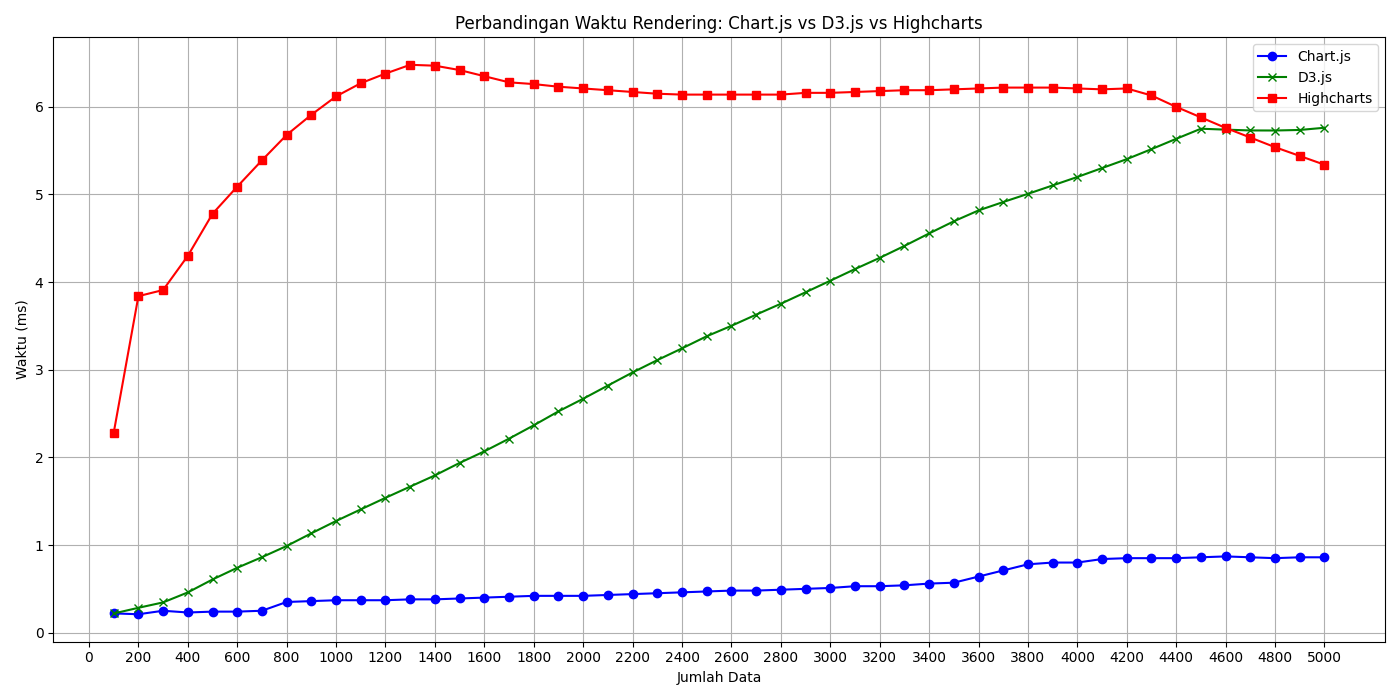
\includegraphics[width=0.8\linewidth]{gambar/Pembahasan/FIX_CPU/Figure_1.png}
	\caption{Grafik Komparasi CPU Pertama}
	\label{Grafik Komparasi CPU Pertama}
\end{figure}
Chart.js menunjukkan waktu render mulai dari sekitar 0.2\% hingga hanya sekitar 0.7\% pada 5000 titik data. D3.js menunjukkan pola kenaikan yang linier dan lebih signifikan dibanding Chart.js. D3 terus mengalami peningkatan penggunaan CPU hingga mencapai hampir 5.9\% pada titik data maksimum. Hal ini menunjukkan D3 membutuhkan lebih banyak resource saat menangani dataset besar. Sementara itu, Highcharts menunjukkan penggunaan CPU yang tinggi sejak awal, mulai dari 2.3\% dan melonjak hingga 6.5\%, sebelum akhirnya menurun sedikit di titik akhir. Penurunan ini bisa terjadi karena mekanisme internal optimasi seperti threshold dan simplifikasi rendering, serta pembatasan otomatis dari browser yang bertujuan menjaga stabilitas dan mencegah aplikasi crash.

Pada eksperimen kedua, pola yang terjadi mirip dengan eksperimen pertama. Nilai Chart.js cenderung stabil, D3 yang meningkat secara signifikan, dan Highcharts yang memiliki waktu render tertinggi. 
	\begin{figure}[H]
	\centering
	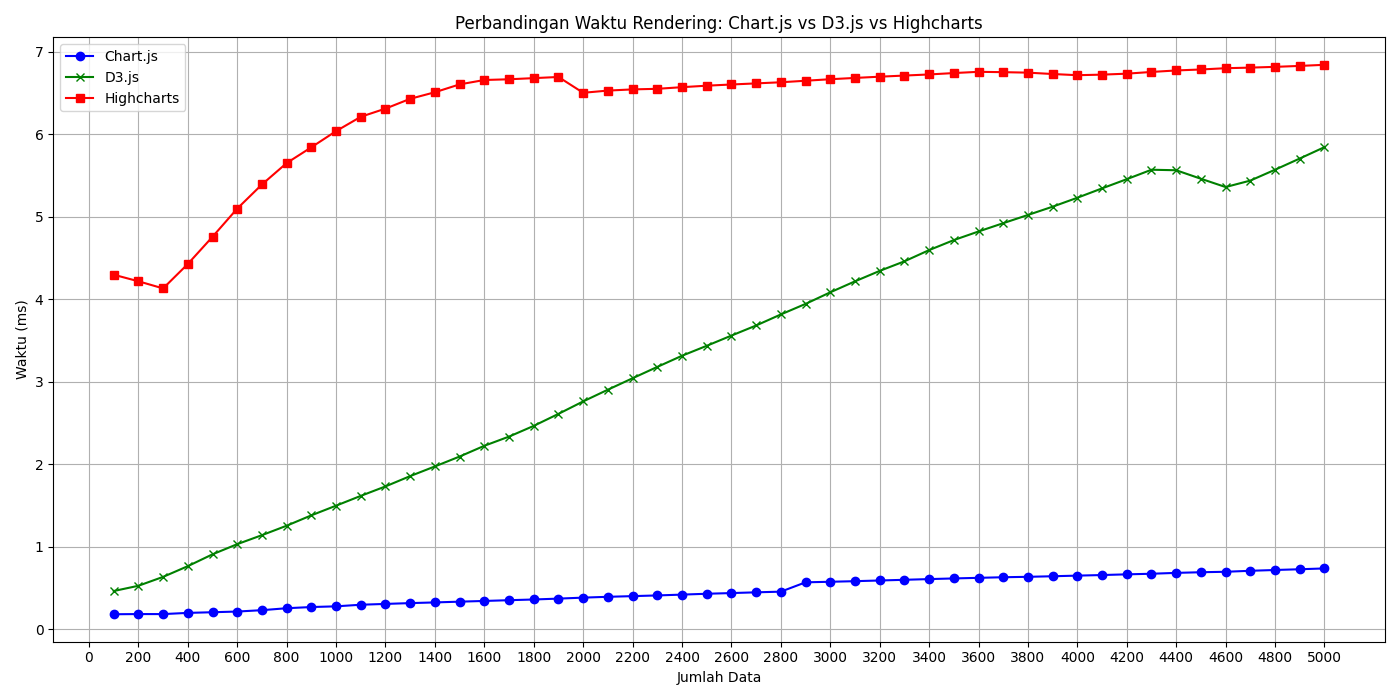
\includegraphics[width=0.8\linewidth]{gambar/Pembahasan/FIX_CPU/Figure_2.png}
	\caption{Grafik Komparasi CPU Kedua}
	\label{Grafik Komparasi CPU Kedua}
\end{figure}
Performa Chart.js tetap konsisten dengan hasil sebelumnya, kembali menunjukkan penggunaan CPU yang rendah dan stabil, bahkan nyaris tidak terpengaruh oleh peningkatan jumlah data. D3 juga menunjukkan tren linier yang mirip dengan sebelumnya, mencapai hampir 5.8\% di 5000 titik data tanpa fluktuasi yang signifikan. Highcharts pada eksperimen ini mengalami penurunan penggunaan CPU di akhir pengujian setelah mencapai puncaknya sekitar 5.2\%, turun menjadi sekitar 4.9\%. Hal ini mengindikasikan adanya stabilisasi pada penggunaan CPU, namun tetap lebih tinggi dibanding dua library lainnya.

Pada eksperimen ketiga, Chart.js masih menunjukkan penggunaan CPU paling kecil, D3 mengalami kenaikan signifikan dan Highcharts memiliki nilai penggunaan CPU tertinggi. 
	\begin{figure}[H]
	\centering
	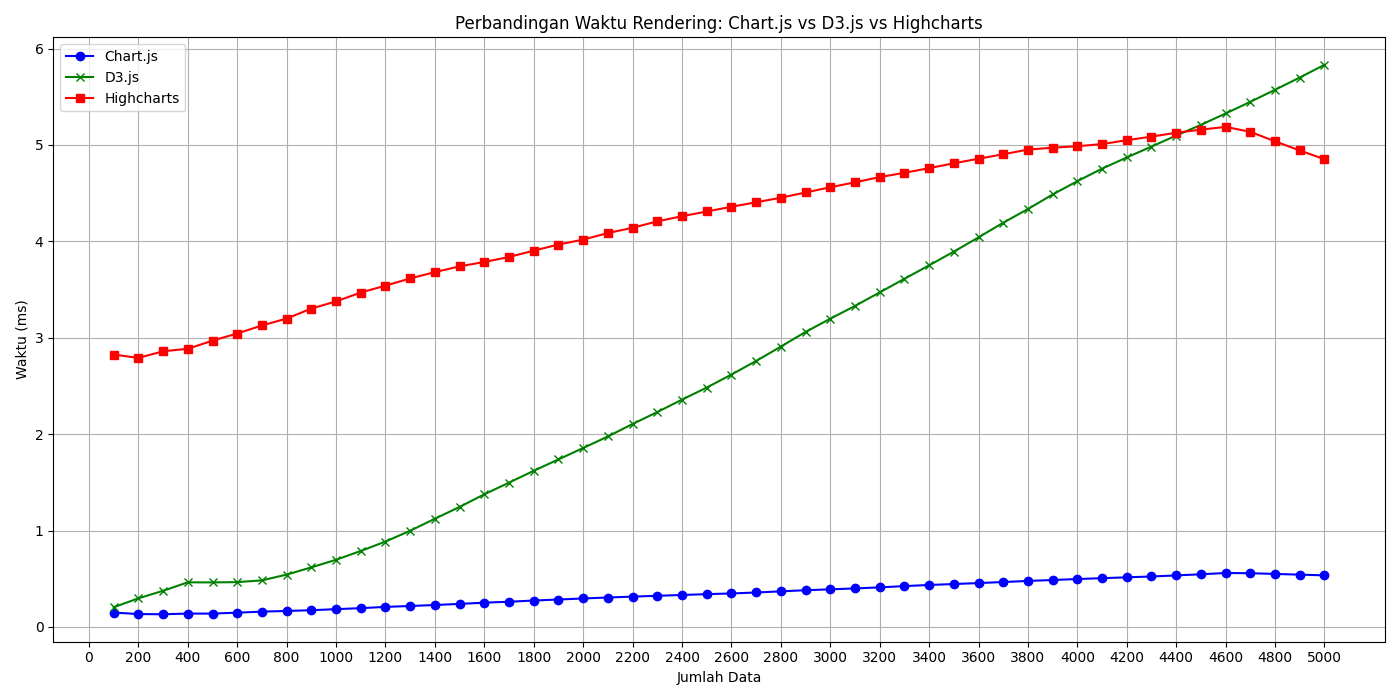
\includegraphics[width=0.8\linewidth]{gambar/Pembahasan/FIX_CPU/Figure_3.png}
	\caption{Grafik Komparasi CPU Ketiga}
	\label{Grafik Komparasi CPU Ketiga}
\end{figure}
Penggunaan CPU oleh Chart.js berkisar di antara 0.2\% hingga 0.6\% secara konsisten. D3.js menunjukkan hasil yang sangat mirip dengan dua eksperimen sebelumnya di mana penggunaan CPU naik secara linier dan mencapai sekitar 5.8\% di titik akhir. Highcharts, memiliki konsumsi CPU yang lebih rendah pada eksperimen ini. Penggunaan CPU berada pada 2,9\% dan mencapai hampir 5,2\% pada 4500 titik data sebelum mengalami penurunan hingga 4,9\%. Hal ini menunjukan untuk menampilkan data dengan  D3 dan Highcharts, diperlukan resource CPU yang besar pula.

\subsection{Alokasi Memori}
\begin{table}[H]
	\centering
	\caption{Perbandingan Penggunaan Memori}
	\small
	\begin{tabular}{|c|ccc|ccc|ccc|}
		\hline
		\textbf{Samples} & \multicolumn{3}{c|}{\textbf{Chart.js}} & \multicolumn{3}{c|}{\textbf{D3.js}} & \multicolumn{3}{c|}{\textbf{Highcharts}} \\
		& \textbf{1st} & \textbf{2nd} & \textbf{3rd} & \textbf{1st} & \textbf{2nd} & \textbf{3rd} & \textbf{1st} & \textbf{2nd} & \textbf{3rd} \\
		\hline
		100   & 56,730  & 59,600  & 56,883  & 108,144 & 52,290  & 108,203 & 97,183  & 70,350  & 83,214 \\
		200   & 57,460  & 66,959  & 58,921  & 112,211 & 60,310  & 112,289 & 106,565 & 92,021  & 91,500 \\
		300   & 66,104  & 74,317  & 60,734  & 120,125 & 68,940  & 120,145 & 111,724 & 108,760 & 100,200 \\
		400   & 70,215  & 81,676  & 62,489  & 128,039 & 73,620  & 128,065 & 114,003 & 134,870 & 117,800 \\
		500   & 74,326  & 89,033  & 64,217  & 132,745 & 86,380  & 136,005 & 116,479 & 140,800 & 120,433 \\
		600   & 78,437  & 96,394  & 65,871  & 143,883 & 95,670  & 143,920 & 126,316 & 150,550 & 124,300 \\
		700   & 82,548  & 103,752 & 67,534  & 161,812 & 105,290 & 161,850 & 135,623 & 157,700 & 130,400 \\
		\vdots & \vdots  & \vdots  & \vdots  & \vdots  & \vdots  & \vdots  & \vdots  & \vdots  & \vdots \\
		4400  & 152,967 & 142,615 & 146,051 & 498,702 & 494,992 & 511,000 & 335,295 & 404,300 & 386,200 \\
		4500  & 155,905 & 143,490 & 146,128 & 499,774 & 473,502 & 515,200 & 338,330 & 407,250 & 388,000 \\
		4600  & 157,111 & 144,365 & 146,152 & 500,344 & 473,790 & 518,000 & 350,158 & 416,000 & 389,200 \\
		4700  & 154,744 & 145,204 & 146,070 & 500,812 & 474,080 & 519,000 & 358,557 & 417,440 & 420,268 \\
		4800  & 156,783 & 148,564 & 146,067 & 501,496 & 487,760 & 519,600 & 365,698 & 417,800 & 390,084 \\
		4900  & 155,316 & 151,889 & 146,070 & 501,855 & 494,600 & 519,900 & 369,709 & 418,450 & 385,700 \\
		5000  & 154,872 & 155,213 & 146,072 & 502,214 & 501,440 & 520,120 & 398,125 & 420,510 & 383,616 \\
		\hline
	\end{tabular}
\end{table}
Pada eksperimen pertama, perbandingan penggunaan memory ditampilkan seperti
berikut
	\begin{figure}[H]
	\centering
	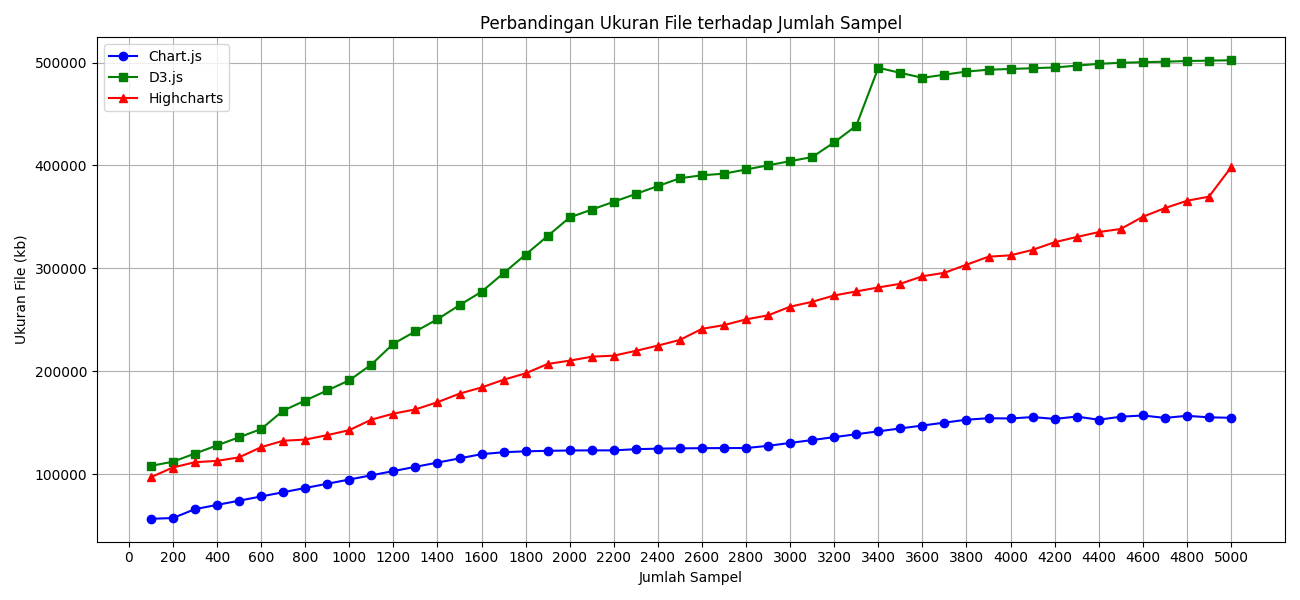
\includegraphics[width=0.8\linewidth]{gambar/Pembahasan/FIX_Memori/Figure_1.png}
	\caption{Grafik Komparasi Memori Pertama}
	\label{Grafik Komparasi Memori Pertama}
\end{figure}

Dari grafik tersebut dapat ditinjau bahwa D3 memiliki penggunaan
memori paling tinggi di antara ketiganya dan terus meningkat secara
signifikan seiring bertambahnya jumlah titik data. Highcharts bada di posisi
tengah, dengan tren peningkatan memori yang konsisten namun tidak setinggi
D3.js. Sementara itu, Chart.js menunjukkan penggunaan memori paling
efisien, dengan peningkatan yang relatif kecil meskipun jumlah titik data
bertambah hingga lebih dari 5000. Hal ini mengindikasikan bahwa Chart.js
lebih optimal untuk aplikasi yang membutuhkan efisiensi memori, terutama
ketika menangani dataset yang besar. D3.js meskipun sangat fleksibel,
cenderung memakan lebih banyak memori, kemungkinan karena struktur dan
proses rendering yang lebih kompleks. 

Pada eksperimen kedua, perbandingan memori ditampilkan seperti berikut
	\begin{figure}[H]
	\centering
	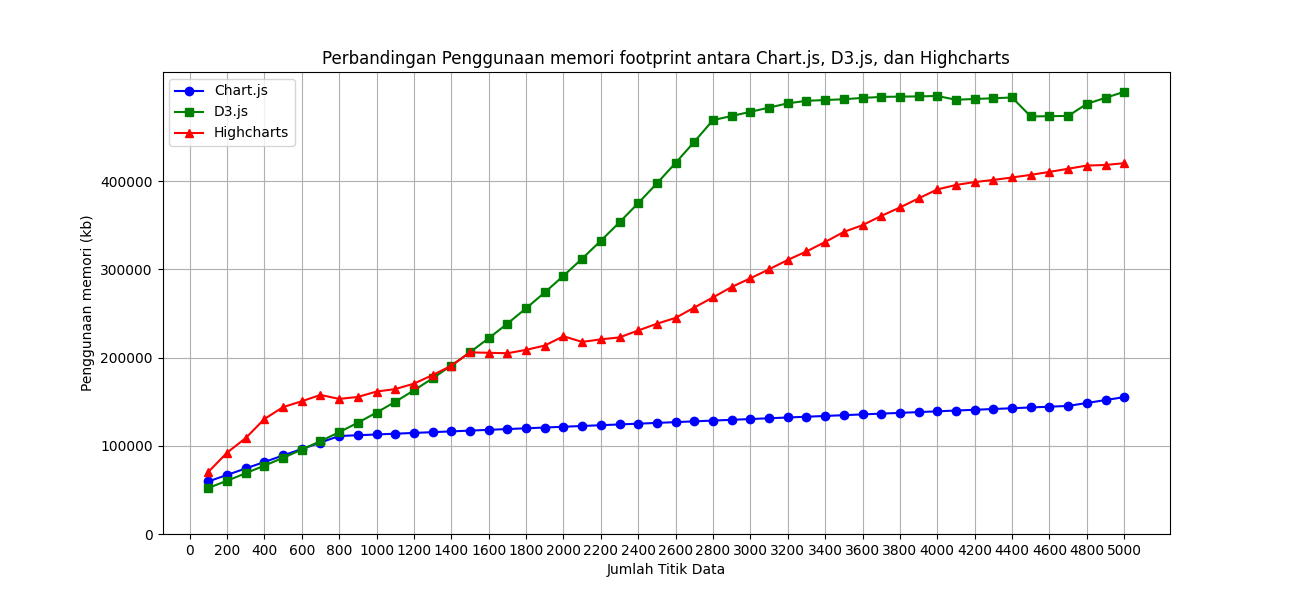
\includegraphics[width=0.8\linewidth]{gambar/Pembahasan/FIX_Memori/Figure_2.png}
	\caption{Grafik Komparasi Memori Kedua}
	\label{Grafik Komparasi Memori Kedua}
\end{figure}
Chart.js masih menunjukkan penggunaan memori yang paling stabil dan
efisien dibandingkan dua library lainnya. Meskipun jumlah titik data
meningkat hingga 5000, kenaikan memori sangat lambat, dengan rata-rata
penggunaan memori di bawah 150 mb. Ini menjadikan Chart.js sangat cocok
untuk aplikasi dengan keterbatasan memori atau kebutuhan visualisasi ringan.
Pada eksperimen ini penggunaan memori oleh D3 dan Highcharts meningkat
secara signifikan.
Pada eksperimen ketiga, Chart.js secara konsisten menghasilkan file
dengan ukuran paling kecil di antara ketiga library.
	\begin{figure}[H]
	\centering
	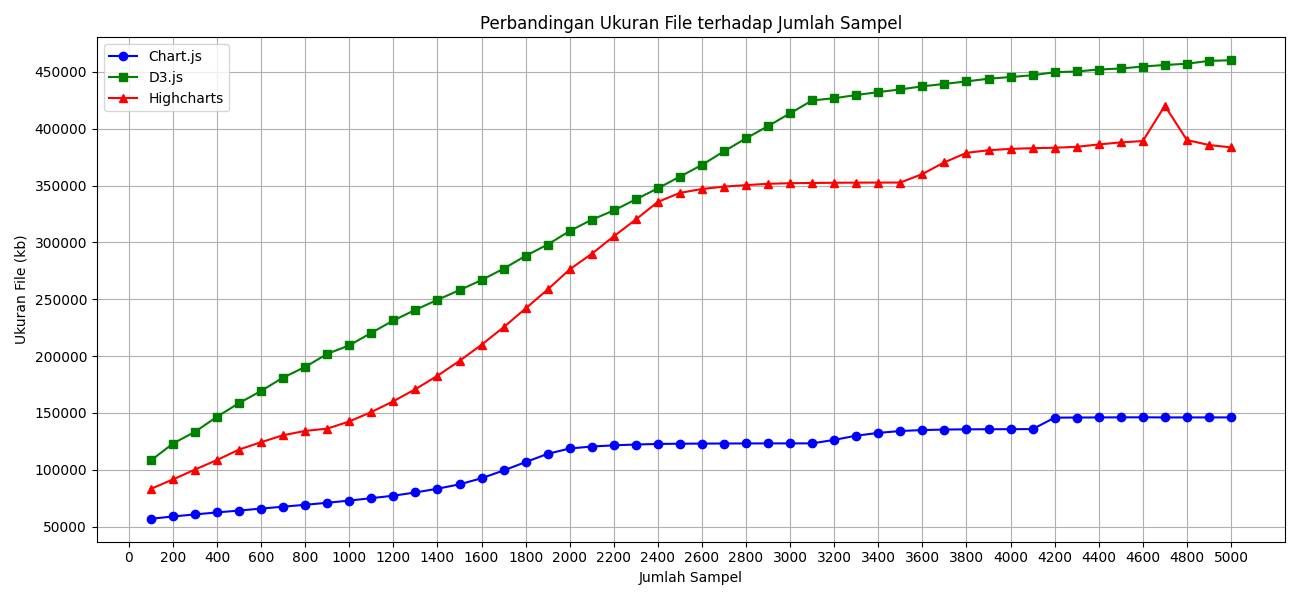
\includegraphics[width=0.8\linewidth]{gambar/Pembahasan/FIX_Memori/Figure_3.png}
	\caption{Grafik Komparasi Memori Ketiga}
	\label{Grafik Komparasi Memori Ketiga}
\end{figure}
Pada percobaan data dengan Chart.js, hingga 5000 sampel, \textit{footprint memory} yang
dihasilkan tidak melebihi 150.000 Kb. Pola kenaikannya juga cukup stabil dan
linear yang menunjukkan efisiensi dalam penyimpanan dan rendering. D3 menghasilkan file dengan ukuran paling besar dan terus meningkat hingga lebih dari 500.000 kb saat
mencapai 5000 data. Ini menunjukkan bahwa meskipun D3 menawarkan
fleksibilitas dan kemampuan kustomisasi yang tinggi, D3 juga memiliki \textit{overhead}
signifikan dalam penyimpanan file. Highcharts berada di posisi tengah antara
D3.js dan Chart.js. Memory footprint yang dihasilkan meningkat secara
eksponensial hingga sekitar 400.000 kb, dan kemudian mengalami sedikit
fluktuasi di titik-titik tertentu, seperti pada sekitar 4700 sampel. Hal ini
menunjukkan bahwa meskipun Highcharts memberikan hasil visualisasi yang
kompleks dan interaktif, penggunaan sumber daya dalam hal memory footprint
masih lebih rendah dibandingkan D3.js, meskipun tetap lebih tinggi dari Chart.js.

